\documentclass[a4paper,12pt,final, openany, titlepage, oneside]{book}

%permette di aggiungere altri pacchetti dai file inclusi
\usepackage[subpreambles]{standalone} 

\usepackage[dvipsnames]{xcolor}
\usepackage{listings}

\lstdefinelanguage{Kotlin}{
	comment=[l]{//},
	commentstyle={\color{gray}\ttfamily},
	emph={[1]first, firstOrNull, forEach, lazy, map, mapNotNull, println},
	emphstyle={[1]\color{OrangeRed}},
	identifierstyle=\color{black},
	keywords={!in, !is, abstract, actual, annotation, as, as?, break, by, catch, class, companion, const, constructor, continue, crossinline, data, delegate, do, dynamic, else, enum, expect, external, false, field, file, final, finally, for, fun, get, if, import, in, infix, init, inline, inner, interface, internal, is, lateinit, noinline, null, object, open, operator, out, override, package, param, private, property, protected, public, receiveris, reified, return, return@, sealed, set, setparam, super, suspend, tailrec, this, throw, true, try, typealias, typeof, val, var, vararg, when, where, while, it},
	keywordstyle={\color{NavyBlue}\bfseries},
	morecomment=[s]{/*}{*/},
	morestring=[b]",
	morestring=[s]{"""*}{*"""},
	ndkeywords={@Deprecated, @JvmField, @JvmName, @JvmOverloads, @JvmStatic, @JvmSynthetic, Array, Byte, Double, Float, Int, Integer, Iterable, Long, Runnable, Short, String, Any, Unit, Nothing, Config, LightEstimationMode, CameraConfigFilter, CameraConfig, FacingDirection, AugmentedFaceMode, AugmentedFace, TrackingState, RegionType, CloudAnchorMode,AugmentedImageDatabase, BitmapFactory, Session, InstantPlacementMode, File, Uri, RecordingConfig },
	ndkeywordstyle={\color{BurntOrange}\bfseries},
	sensitive=true,
	stringstyle={\color{ForestGreen}\ttfamily},
	emph={[2]FRONT,MESH3D,ENVIRONMENTAL\_HDR,AMBIENT\_INTENSITY, DISABLED,FOREHEAD\_LEFT,FOREHEAD\_RIGHT,NOSE\_TIP, TRACKING, ENABLED, LOCAL\_Y\_UP},
	emphstyle={[2]\color{Purple}\ttfamily},
}

\definecolor{lightgrey}{RGB}{230,237,244}

\lstset{
	basicstyle=\scriptsize\sffamily\color{black},
	backgroundcolor=\color{lightgrey},
	frame=single,
	numbers=left,
	numbersep=5pt,
	numberstyle=\tiny\color{gray},
	showspaces=false,
	showstringspaces=false,
	tabsize=1,
	texcl=true,
	captionpos=b,
	breaklines=true
}





%impostazioni lingua
\usepackage[T1]{fontenc}
\usepackage[utf8]{inputenc}
\usepackage[english,italian]{babel}

%sistema i margini
\usepackage{geometry}
\geometry{a4paper,top=2.2cm,bottom=2.2cm,left=3cm,right=3cm, heightrounded}

%interlinea 1.5
\usepackage{setspace}
\onehalfspacing

%gestione delle testatine
\usepackage{fancyhdr}
\pagestyle{fancy}
\lhead{}
\chead{}
\rhead{Google ARCore}
\lfoot{}
\cfoot{\thepage}
\rfoot{}
\renewcommand{\headrulewidth}{0.4pt}

%formattazione titoli paragrafo
\usepackage{titlesec}
\titleformat{\chapter}[block]{\normalfont\huge\bfseries}{\thechapter.}{0.7em}{\huge}

\usepackage{caption}


\usepackage[autostyle,italian=guillemets]{csquotes}
\usepackage[sorting = nty,style=numeric,citestyle=numeric-comp,backend=biber]{biblatex}

\addbibresource{bibliografia.bib}

%collegamenti ipertestuali
%\usepackage{hyperref}

%genera testo casuale
\usepackage{lipsum}

\begin{document}
	
	
	\frontmatter
	\documentclass[crop=false]{standalone}

\usepackage{frontespizio}

\begin{document}
	\begin{frontespizio}
		\Preambolo{\renewcommand{\fronttitlefont}{%
				\fontsize{22}{22}\bfseries}}
		
		\Universita{Padova}
		\Logo[3cm]{./resources/images/loghi.jpg}
		\Dipartimento{Ingegneria dell'Informazione}
		\Corso[Laurea]{Ingegneria Informatica}
		\Titolo{Google ARCore}
		%aggiunge più candidati
		\NCandidati{}
		%elimina il carattere ":"
		\Punteggiatura{}
		\Preambolo{\renewcommand{\frontcandidatesep}{0.5cm}}
		\Candidato[1216433]{Marco Vettore}
		\Candidato[1227153]{Alberto Varini}
		\Candidato[1219603]{Mattia Tamiazzo}
		\Rientro{1cm}
		\Annoaccademico{2021-2022}
		\Margini{1.5cm}{1cm}{1.5cm}{1cm}
	\end{frontespizio}
\end{document}

	\documentclass[crop=false]{standalone}

\begin{document}
	\tableofcontents
\end{document}
	
	
	\mainmatter
	% Mattia
	\documentclass[crop=false, class=book]{standalone}

%impostazioni lingua
\usepackage[T1]{fontenc}
\usepackage[utf8]{inputenc}
\usepackage[english,italian]{babel}

%sistema i margini
\usepackage{geometry}
\geometry{a4paper,top=2.2cm,bottom=2.2cm,left=3cm,right=3cm, heightrounded}

%interlinea 1.5
\usepackage{setspace}
\onehalfspacing

%gestione delle testatine
\usepackage{fancyhdr}
\pagestyle{fancy}
\lhead{}
\chead{}
\rhead{Titolo}
\lfoot{}
\cfoot{\thepage}
\rfoot{}
\renewcommand{\headrulewidth}{0.4pt}

%formattazione titoli paragrafo
\usepackage{titlesec}
\titleformat{\chapter}[block]{\normalfont\huge\bfseries}{\thechapter.}{0.7em}{\huge}

%pacchetti per i riferimenti in bibliografia
\usepackage[autostyle,italian=guillemets]{csquotes}
\usepackage[sorting=none,style=numeric,citestyle=numeric-comp,backend=biber]{biblatex}

%risorsa che contiene la bibliografia
\addbibresource{./../bibliografia.bib}



\begin{document}
	\chapter{Introduzione}
	La Realtà Aumentata (Augmented Reality - \emph{AR}) è una tecnologia che permette di compiere esperienze interattive, in cui l'ambiente reale viene arricchito da contenuti virtuali. Similmente alla realtà virtuale, vengono creati elementi grafici sintetici con cui l'utente può interagire attraverso i sensi. Tuttavia, come spiegato in \cite{bimber2005spatial}, nell'AR l'ambiente reale gioca un ruolo fondamentale: lo scopo della realtà aumentata è proprio cercare di collegare il mondo reale con quello virtuale.
	\\
	L'AR viene definita in \cite{azuma1997survey} come un sistema che incorpora tre caratteristiche principali: la combinazione tra reale e virtuale, l'interazione real-time e la rappresentazione 3D. 
	
	\section{Storia}
	Il primo rudimentale sistema di realtà aumentata è stato creato da Ivan Sutherland \cite{sutherland1968head} nel 1968. Esso era composto da un display ottico trasparente che veniva montato sulla testa e che poteva mostrare semplici immagini in tempo reale. Nel 1993 George Fitzmaurice ha creato \textit{Chameleon} \cite{fitzmaurice1993situated}, un dispositivo che tramite un piccolo schermo collegato a una videocamera poteva essere orientato per esplorare uno spazio virtuale 3D. Simile al prototipo di Fitzmaurice, nel 1995 Jun Rekimoto e Katashi Nagao creano \textit{NaviCam} \cite{rekimoto1995world}, che prendendo in input un flusso video poteva riconoscere in real-time dei marcatori colorati e sovrapporre al video delle informazioni testuali. 
	\\
	Dal 2000 vengono creati altri primi sistemi di realtà aumentata, con applicazioni soprattutto a giochi interattivi, come ad esempio l'estensione \textit{ARQuake} \cite{thomas2000arquake} o \textit{Human Pacman} \cite{cheok2003human}, ancora vincolati alle scarse prestazioni dei dispositivi mobili. Solo con l'aggiunta ai cellulari della fotocamera, e poi di schermi touch, vengono quindi create le prime applicazioni commerciali in grado di sfruttare le potenzialità della realtà aumentata. Ne sono esempi \textit{AR Tennis} \cite{henrysson2006ARtennis}, primo gioco in AR collaborativo per cellulare, e \textit{ARhrrrr!}, primo gioco mobile in realtà aumentata con contenuti grafici di alta qualità. Vengono quindi sviluppate le prime librerie software per la realtà aumentata, come \textit{ARToolKit}, implementata prima in linguaggio C e poi in C++ nelle versioni più recenti, \textit{OpenCV}, che possiede anche funzionalità per l'AR, e dal 2018 la libreria per Android \textit{ARCore} di Google.
	
	\section{Applicazioni}	
	Le applicazioni della realtà aumentata possono riguardare diversi ambiti, ai quali questa tecnologia può apportare benefici economici o qualitativi, oppure creare servizi innovativi \cite{carmigniani2011augmented}. 
	\\
	In particolare, nel corso degli anni la tecnologia AR è stata usata per scopi pubblicitari e commerciali, quali la prova di capi d'abbigliamento senza doverli indossare o l'integrazione al marketing cartaceo di video promozionali tramite riconoscimento delle immagini, o per l'intrattenimento, come nello sviluppo di videogiochi. Trova inoltre applicazioni nella produzione industriale, in cui vengono sovrapposte all'area di lavoro istruzioni virtuali, nell'ambito militare, come l'addestramento al volo dei piloti, o per la formazione e la pratica sanitaria.
\end{document}
	\documentclass[crop=false, class=book]{standalone}




\begin{document}
	\chapter{Realtà aumentata}
	La Realtà Aumentata (Augmented Reality - \emph{AR}) è una tecnologia che permette di compiere esperienze interattive, in cui l'ambiente reale viene arricchito da contenuti virtuali. Similmente alla realtà virtuale, vengono creati elementi grafici sintetici con cui l'utente può interagire attraverso i sensi. Tuttavia, come spiegato in \cite{bimber2005spatial}, nell'AR l'ambiente reale gioca un ruolo fondamentale: lo scopo della realtà aumentata è proprio cercare di collegare il mondo reale con quello virtuale.
	\\
	L'AR viene definita in \cite{azuma1997survey} come un sistema che incorpora tre caratteristiche principali: la combinazione tra reale e virtuale, l'interazione real-time e la rappresentazione 3D. 
	
	\section{Storia}
	Il primo rudimentale sistema di realtà aumentata è stato creato da Ivan Sutherland \cite{sutherland1968head} nel 1968. Esso era composto da un display ottico trasparente che veniva montato sulla testa e che poteva mostrare semplici immagini in tempo reale. Nel 1993 George Fitzmaurice ha creato \textit{Chameleon} \cite{fitzmaurice1993situated}, un dispositivo che tramite un piccolo schermo collegato a una videocamera poteva essere orientato per esplorare uno spazio virtuale 3D. Simile al prototipo di Fitzmaurice, nel 1995 Jun Rekimoto e Katashi Nagao creano \textit{NaviCam} \cite{rekimoto1995world}, che prendendo in input un flusso video poteva riconoscere in real-time dei marcatori colorati e sovrapporre al video delle informazioni testuali. 
	\\
	Dal 2000 vengono creati altri primi sistemi di realtà aumentata, con applicazioni soprattutto a giochi interattivi, come ad esempio l'estensione \textit{ARQuake} \cite{thomas2000arquake} o \textit{Human Pacman} \cite{cheok2003human}, ancora vincolati alle scarse prestazioni dei dispositivi mobili. Solo con l'aggiunta ai cellulari della fotocamera, e poi di schermi touch, vengono quindi create le prime applicazioni commerciali in grado di sfruttare le potenzialità della realtà aumentata. Ne sono esempi \textit{AR Tennis} \cite{henrysson2006ARtennis}, primo gioco in AR collaborativo per cellulare, e \textit{ARhrrrr!}, primo gioco mobile in realtà aumentata con contenuti grafici di alta qualità. Vengono quindi sviluppate le prime librerie software per la realtà aumentata, come \textit{ARToolKit}, implementata prima in linguaggio C e poi in C++ nelle versioni più recenti, \textit{OpenCV}, che possiede anche funzionalità per l'AR, e dal 2018 la libreria per Android \textit{ARCore} di Google.
	
	\section{Applicazioni}	
	Le applicazioni della realtà aumentata possono riguardare diversi ambiti, ai quali questa tecnologia può apportare benefici economici o qualitativi, oppure creare servizi innovativi \cite{carmigniani2011augmented}. 
	\\
	In particolare, nel corso degli anni la tecnologia AR è stata usata per scopi pubblicitari e commerciali, quali la prova di capi d'abbigliamento senza doverli indossare o l'integrazione al marketing cartaceo di video promozionali tramite riconoscimento delle immagini, o per l'intrattenimento, come nello sviluppo di videogiochi. Trova inoltre applicazioni nella produzione industriale, in cui vengono sovrapposte all'area di lavoro istruzioni virtuali, nell'ambito militare, come l'addestramento al volo dei piloti, o per la formazione e la pratica sanitaria.
	
	 
\end{document}
	\documentclass[crop=false, class=book]{standalone}


\begin{document}
	\chapter{Funzioni fondamentali}
	\textbf{TODO creazione di sessione?}
	Nel seguente capitolo vengono 
	
	 
\end{document}
	
	% Alberto
	\documentclass[crop=false, class=book]{standalone}

%impostazioni lingua
\usepackage[T1]{fontenc}
\usepackage[utf8]{inputenc}
\usepackage[english,italian]{babel}

%sistema i margini
\usepackage{geometry}
\geometry{a4paper,top=2.2cm,bottom=2.2cm,left=3cm,right=3cm, heightrounded}

%interlinea 1.5
\usepackage{setspace}
\onehalfspacing

%gestione delle testatine
\usepackage{fancyhdr}
\pagestyle{fancy}
\lhead{}
\chead{}
\rhead{Titolo}
\lfoot{}
\cfoot{\thepage}
\rfoot{}
\renewcommand{\headrulewidth}{0.4pt}

%formattazione titoli paragrafo
\usepackage{titlesec}
\titleformat{\chapter}[block]{\normalfont\huge\bfseries}{\thechapter.}{0.7em}{\huge}

%pacchetti per i riferimenti in bibliografia
\usepackage[autostyle,italian=guillemets]{csquotes}
\usepackage[style=numeric,citestyle=numeric-comp,backend=biber]{biblatex}

%risorsa che contiene la bibliografia
\addbibresource{./../bibliografia.bib}

\usepackage{lipsum}
\usepackage{graphicx}
\usepackage[italian]{varioref}
\usepackage{copyrightbox}

\begin{document}

	\chapter{Motion tracking}
	
		ARCore usa un processo chiamato \emph{Simultaneous localization and mapping (SLAM)} per determinare lo stato del
		dispositivo che si trova all'interno di un ambiente sconosciuto. Questo stato è descritto dalla sua posa (posizione 
		e orientazione) che viene stimata attraverso prestazioni di odometria eccezionali e rilevazione di punti 						caratteristici. Con odometria si intende l'uso di dati ricavati da sensori di movimento che permettono di valutare il 			cambiamento della posizione nel tempo. Nel caso degli smartphone viene utilizzato il sensore IMU che 							rileva misure inerziali come la velocita, accelerazione e posizione. La rilevazione di punti caratteristici è 					l'individuazione di immagini con caratteristiche differenti che consentono al dispositivo di calcolare la sua posizione 		relativa. Questi punti di riferimento insieme alle misurazioni ricavate dai sensori permettono di avere una 					buona stima della posa e di ricavare la rappresentazione di una mappa dell'ambiente circostante. Tuttavia, 						il movimento sequenziale stimato dallo SLAM include un certo margine di errore che si accumula nel tempo causando 				una notevole deviazione dai valori reali. Una soluzione che può essere adottata per risolvere questo 							problema consiste nel considerare come punto di riferimento un luogo visitato in precedenza di cui si sono 						memorizzate le sue caratteristiche. Grazie alle informazioni di questo luogo è possibile minimizzare l'errore nella 			stima della posa.\\
		I contenuti virtuali possono essere renderizzati nella giusta prospettiva allineando la posa della telecamera virtuale 			con quella calcolata da ARCore. Il contenuto virtuale sembra reale perchè è sovrapposto all'immagine ottenura dalla 			fotocamera del dispositivo.
	
\end{document}
	
	% Marco 
	\documentclass[crop=false, class=book]{standalone}

%impostazioni lingua
\usepackage[T1]{fontenc}
\usepackage[utf8]{inputenc}
\usepackage[english,italian]{babel}

%sistema i margini
\usepackage{geometry}
\geometry{a4paper,top=2.2cm,bottom=2.2cm,left=3cm,right=3cm, heightrounded}

%interlinea 1.5
\usepackage{setspace}
\onehalfspacing

%formattazione titoli paragrafo
\usepackage{titlesec}
\titleformat{\chapter}[block]{\normalfont\huge\bfseries}{\thechapter.}{0.7em}{\huge}

%pacchetti per i riferimenti in bibliografia
\usepackage[autostyle,italian=guillemets]{csquotes}
\usepackage[sorting=none,style=numeric,citestyle=numeric-comp,backend=biber]{biblatex}
\usepackage[pdftex]{graphicx} 

%risorsa che contiene la bibliografia
\addbibresource{./../../bibliografia.bib}

\usepackage{copyrightbox}



\begin{document}
	\section{Comprensione Ambientale}
	ARCore ha a disposizione funzione di comprensione dell’ambiente che gli consente di capire cosa circonda il dispositivo. Questa funzione è basata sulla ricerca di piani e vari punti caratteristici dell’ambiente.
	
	ARCore si concentra nel trovare dei punti caratteristici posati lungo piani verticali e orizzontali così da riuscire a calcolare la posizione dei piani attraverso dei calcoli tra i sensori del dispositivo uniti al tracciamento dei punti caratteristici nell’immagine. 
	
	Inoltre, questa libreria è in grado di rilevare i bordi dei piani e utilizzare tutte queste informazioni per poter posizionare degli oggetti virtuali su di essi.
	
	Poiché ARCore basa la sua comprensione dell’ambiente su dei punti caratteristici, le superfici senza texture come un pavimento o un muro bianco potrebbero non essere rilevate facilmente.

	\begin{center}
		\begin{figure}
			\centering
			\copyrightbox[l]{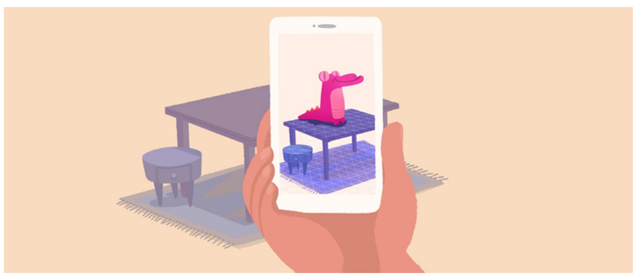
\includegraphics[width=0.9\textwidth]{./../../resources/images/EnvironmentalUnderstanding/env_understanding.png}}%
			{Fonte: \url{https://developers.google.com}}
			\caption{Esempio degli effetti prodotti dagli oggetti nell'ambiente.}
			\label{fig:env_und}
		\end{figure}
	\end{center}
	
	Nell'applicazione che abbiamo sviluppato questa abilità diventa fondamentale.L'oggetto posizionato viene scalato in base all'ambiente così da renderlo più realistico.
	
	\begin{center}
		\begin{figure}
		\centering
		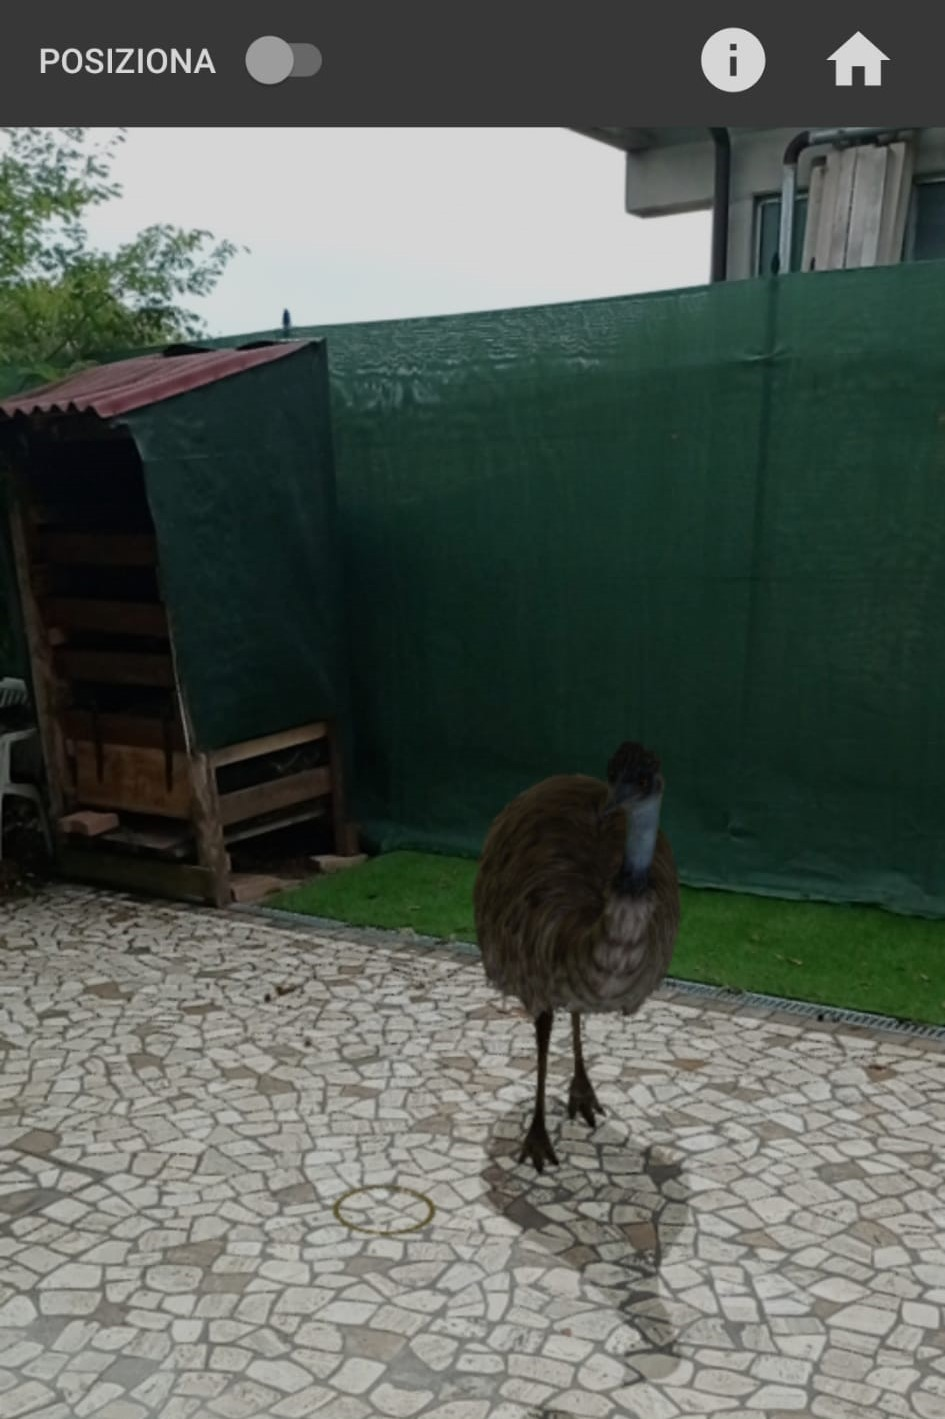
\includegraphics[scale=0.22]{EUImg1.jpeg} 
		\caption{Esempio dell'immersione dell'oggetto nella nostra 	applicazione nell'ambiente}
	\end{figure}
	
	\end{center}

\end{document}
	
	% Mattia
	\documentclass[crop=false, class=book]{standalone}


%pacchetto per immagini
\usepackage{graphicx}

\usepackage[italian]{varioref}
\usepackage{copyrightbox}
\usepackage{url}

\begin{document}
	\section{Light Estimation}
	\label{sec:light_est}
	Nel rendering in realtà aumentata è importante che gli oggetti virtuali siano il più possibile integrati con l'ambiente circostante. Una delle caratteristiche principali che permette all'occhio umano di percepire la posizione di un oggetto nello spazio è la luce, cioè il modo in cui esso viene illuminato e l'ombra che proietta. 
	Proprio per questo motivo, il framework ARCore mette a disposizione il \textit{Light Estimation API}, che fornisce informazioni dettagliate riguardo l'illuminazione della scena, come spiegato nella documentazione ufficiale \cite{google2022light}.
	Tali informazioni sono necessarie per imitare i vari effetti che producono gli oggetti reali quando colpiti da una fonte di luce, che sono descritti dalla figura~\vref{fig:light_effects}:
	\begin{itemize}
		\item le \textbf{ombre} (\textit{shadows}), che sono direzionali e suggeriscono dove è collocata la fonte di luce;
		\item l'\textbf{ombreggiatura} (\textit{shading}), cioè l'intensità della luce che colpisce una certa faccia dell'oggetto;
		\item la \textbf{lumeggiatura} (\textit{specular highlight}), la macchia luminosa che compare su un oggetto lucido quando viene illuminato;
		\item la \textbf{riflessione} (\textit{reflection}), che può essere con proprietà speculari per oggetti completamente lucidi, come ad esempio uno specchio, oppure di diffusione, non dando un chiaro riflesso dell'ambiente circostante. 
	\end{itemize}
	
	\begin{figure}
		\centering
		\copyrightbox[l]{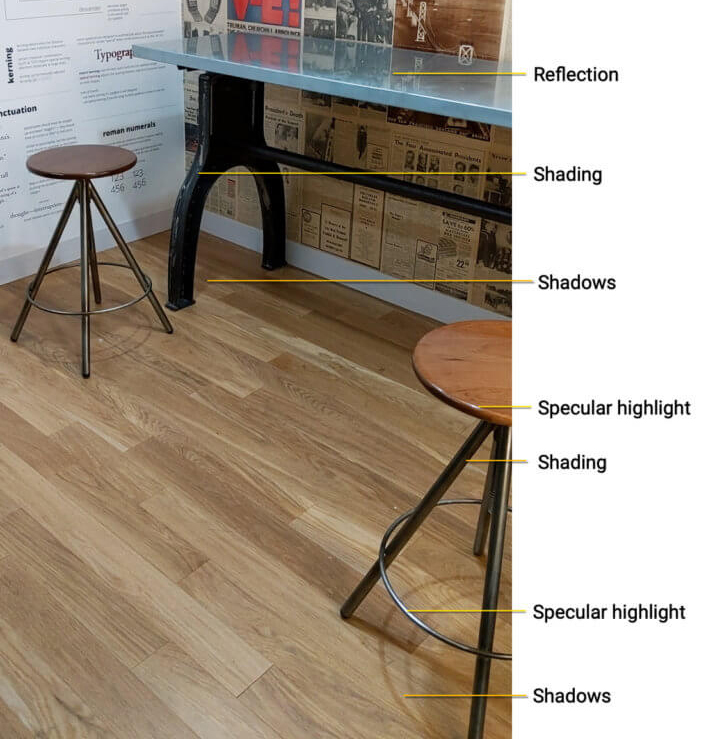
\includegraphics[width=0.5\textwidth]{./resources/images/light_estimation/light_effects}}%
			{Fonte: \url{https://developers.google.com}}
		\caption{Esempio degli effetti prodotti dagli oggetti quando sono illuminati.}
		\label{fig:light_effects}
	\end{figure}
    \noindent
	Le modalità per la gestione della stima della luce sono due, l'\textit{Environmental HDR mode} e l'\textit{Ambient intensity mode}. Durante la configurazione della sessione ARCore può essere scelta una delle due modalità, oppure disabilitare la stima della luce, come mostra il listing~\vref{lst:le_session} tratto dalla guida ufficiale.
	\\
	
	\begin{center}
		\begin{minipage}{0.95\textwidth}
			\begin{lstlisting}[caption={Configurazione della modalità di stima della luce.}, label={lst:le_session}, language=Kotlin]
			// Configura la sessione in modalità \verb|ENVIRONMENTAL_HDR|
			val config : Config = session.config
			config.lightEstimationMode = LightEstimationMode.ENVIRONMENTAL_HDR
			session.configure(config)
			
			// Configura la sessione in modalità \verb|AMBIENT_INTENSITY|
			val config : Config = session.config
			config.lightEstimationMode = LightEstimationMode.AMBIENT_INTENSITY
			session.configure(config)
				
			// Configura la sessione disabilitando la Light Estimation API
			val config : Config = session.config
			config.lightEstimationMode = LightEstimationMode.DISABLED
			session.configure(config)
			\end{lstlisting}
		\end{minipage}
	\end{center}


	

	\subsection{Environmental HDR mode}
		La modalità \textit{Environmental HDR} combina tre diverse API per replicare la luce reale, come descritti dalla figura~\vref{fig:env_HDR}.
	
		\paragraph*{Main Directional Light}
			Questa API calcola la direzione e l'intensità della fonte di luce principale, permettendo di posizionare correttamente l'ombra e la lumeggiatura dell'oggetto virtuale. Inoltre, questa funzionalità permette ad entrambi questi effetti ottici di venire corretti se cambia la posizione relativa dell'oggetto rispetto la fonte di luce
		
		\paragraph*{Ambient Spherical Harmonics}
			Questa funzionalità permette di rappresentare la luce ambientale della scena, parametrizzando l'intensità della luce proveniente dalle varie direzioni.
		
	
		\paragraph*{HDR Cubemap}
			Essa permette di riprodurre la riflessione di oggetti con superfici lucide. Tramite questa API viene modificata anche l'ombreggiatura e il colore dell'oggetto, che dipenderanno dalla tonalità dell'ambiente circostante.
	
		\begin{figure}
			\centering
			\copyrightbox[l]{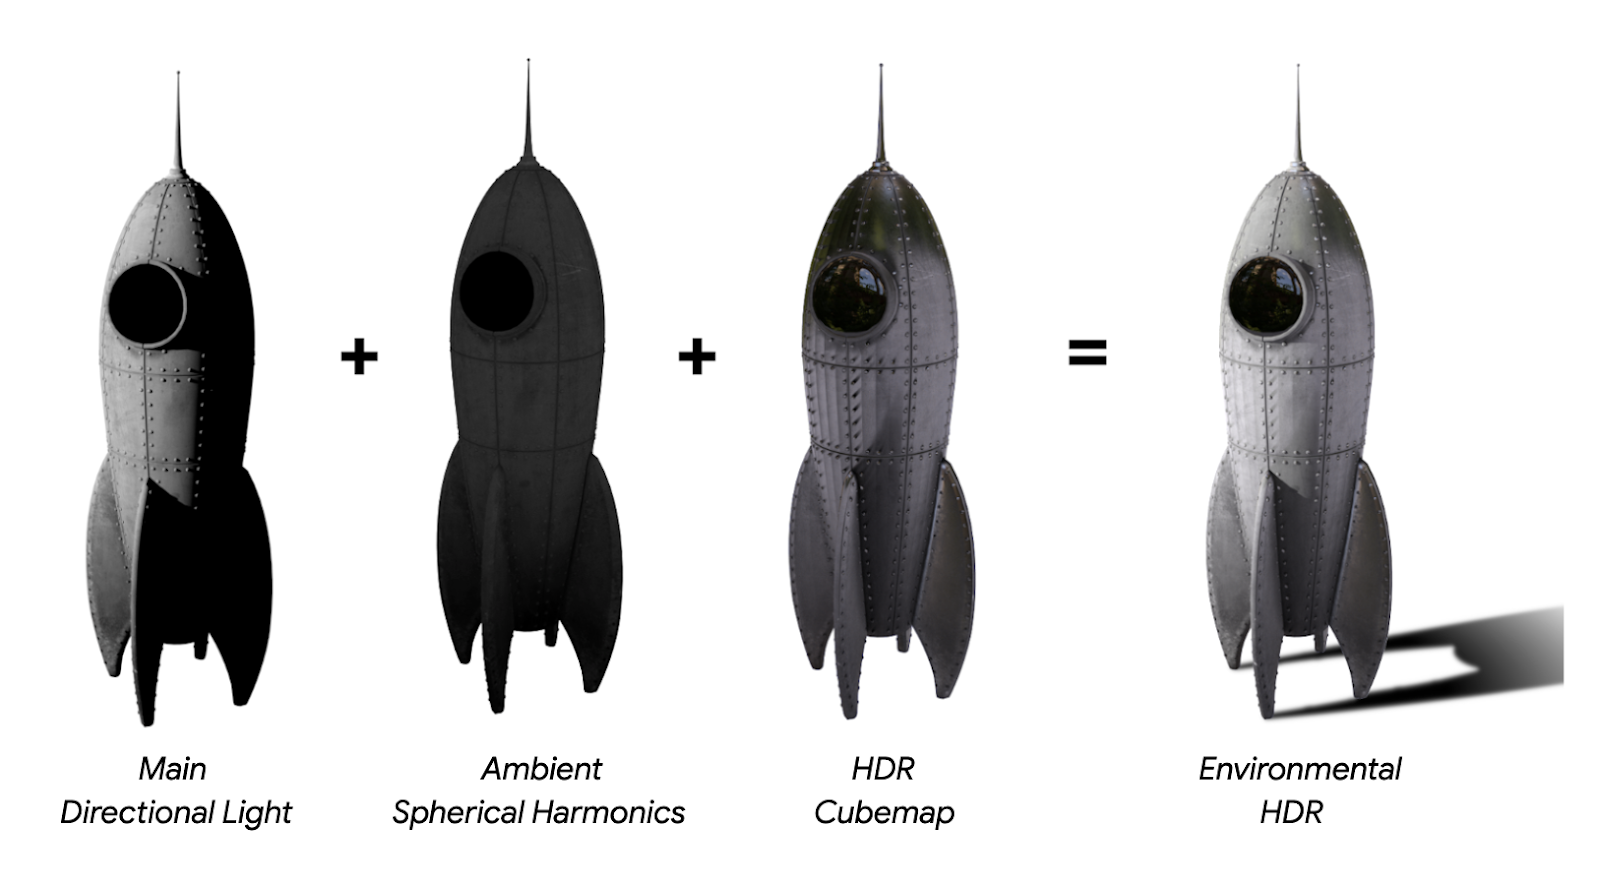
\includegraphics[width=0.8\textwidth]{./resources/images/light_estimation/env_HDR}}%
			{Fonte: \url{https://developers.googleblog.com}}
			\caption{Composizione della modalità Environmental HDR.}
			\label{fig:env_HDR}
		\end{figure}
	
	\subsection{Ambient intensity mode}
		La modalità \textit{Ambient intensity} determina l'intensità media dei pixel e la correzione del colore di una data immagine. Dopo aver filtrato l'intensità media di un insieme di pixel e il bilanciamento del bianco per ogni frame, vengono corretti la luce e il colore dell'oggetto virtuale, affinché si integri meglio con la scena \cite{suonsivu2020rgbd}. Questa modalità può essere utilizzata se la stima della luce non è critica, come per oggetti che possiedono già una propria illuminazione integrata.
	
	
\end{document}
	
	
	% Alberto
	\documentclass[crop=false, class=book]{standalone}

%impostazioni lingua
\usepackage[T1]{fontenc}
\usepackage[utf8]{inputenc}
\usepackage[english,italian]{babel}

%sistema i margini
\usepackage{geometry}
\geometry{a4paper,top=2.2cm,bottom=2.2cm,left=3cm,right=3cm, heightrounded}

%interlinea 1.5
\usepackage{setspace}
\onehalfspacing

%gestione delle testatine
\usepackage{fancyhdr}
\pagestyle{fancy}
\lhead{}
\chead{}
\rhead{Titolo}
\lfoot{}
\cfoot{\thepage}
\rfoot{}
\renewcommand{\headrulewidth}{0.4pt}

%formattazione titoli paragrafo
\usepackage{titlesec}
\titleformat{\chapter}[block]{\normalfont\huge\bfseries}{\thechapter.}{0.7em}{\huge}

%pacchetti per i riferimenti in bibliografia
\usepackage[autostyle,italian=guillemets]{csquotes}
\usepackage[style=numeric,citestyle=numeric-comp,backend=biber]{biblatex}

%risorsa che contiene la bibliografia
\addbibresource{./../bibliografia.bib}

\usepackage{lipsum}
\usepackage{graphicx}
\usepackage[italian]{varioref}
\usepackage{copyrightbox}

\begin{document}
		
	\chapter{Depth understanding}
	
		ARCore Depth API  permette agli sviluppatori di generare mappe di profondità attraverso l'uso di algoritmi di 					profondità del movimento. Una mappa di profondità offre una visualizzazione in 3D del mondo reale, ogni pixel è 				associato alla distanza dalla scena e attraverso l'uso di colori differenti è possibile riconoscere quali aree dello 			spazio sono più vicine al dispositivo. Quando viene avviata una nuova sessione ARCore il display dello smartphone è 			nero, ma non appena si effettua un piccolo movimento la profondità viene rilevata. La stima della profondità è ricavata 		attraverso il movimento dello smartphone. Quando si progettano delle applicazioni che si concentrano sulla profondità 			bisogna considerare che la profondità viene calcolata meglio quando la scena rimane la stessa con piccoli spostamenti. 			Il dispositivo ha bisogno di muoversi un pò per generare la profondità. Un altro fattore da prendere in considerazione 			è quando l'utente compie lunghi spostamenti; in questo caso la stima della profondità arriva fino a 8 metri ma la 				migliore accuratezza si ha tra 0 e 5 metri.\\
		Per ottimizzare ulteriormente le funzionalità offerte da depth API è stato effettuato un uso selettivo del machine 				learning
		 Le principale funzionalità offerte da depth API sono tre:
		\begin{itemize}
			\item[•] \textbf{Copertura dei contenuti}: permette di posizionare accuratamente dei contenuti virtuali di fronte o dietro degli oggetti reali.
			\item[•] \textbf{Immersione}: permette di decorare una scena con oggetti virtuali che interagiscono tra di loro.
			\item[•] \textbf{Interazione}: i contenuti virtuali sono in grado di interagire con il mondo reale attraverso cambiamenti fisici e collisioni.
		\end{itemize}
		
		
		\section{Sessione ARCore con depth API}
		
		Prima di iniziare una nuova sessione ARCore è necessario controllare se il dispositivo supporta depth API. A volte 				questa opzione può essere disattivata oppure non supportata nonostante il dispositivo supporti ARCore. Dopo aver 				definito la sessione con le opportune configurazioni è possibile controllare se il dispositivo e la fotocamera 					supportano una determinata modalità di profondità invocando il metodo \textit{isDepthModeSupported(Config.DepthMode 			mode)} sull'istanza della sessione. Se la modalità è supportata viene configurata la sessione e sarà possibile 					sfruttare depth API. (Esempio\vref{fig: Controllo supporto depth API})\\
		
		\begin{figure}
			\centering
			\copyrightbox[0.5]{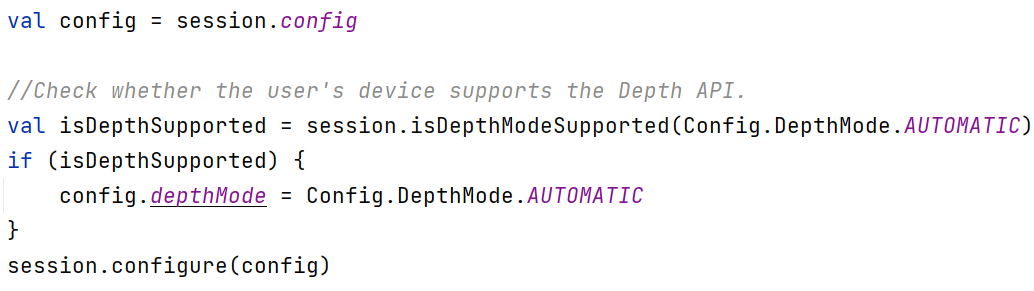
\includegraphics[width=0.8\textwidth]{../../resources/images/depthAPI/depthAPI1.PNG}}%
			{Fonte: \url{https://developers.google.com/ar/develop/java/depth/developer-guide}}
			\caption{Controllo supporto depth API}
			\label{fig: Controllo supporto depth API}
		\end{figure}
		
		\begin{flushleft}
		Per ottenere l'immagine di profondità relativa al frame corrente viene invocato il metodo 										\textit{acquireDepthImage16Bits()}. (Esempio \vref{fig: Immagine di profondità})\\
		\end{flushleft}
		\begin{figure}
			\centering
			\copyrightbox[0.5]{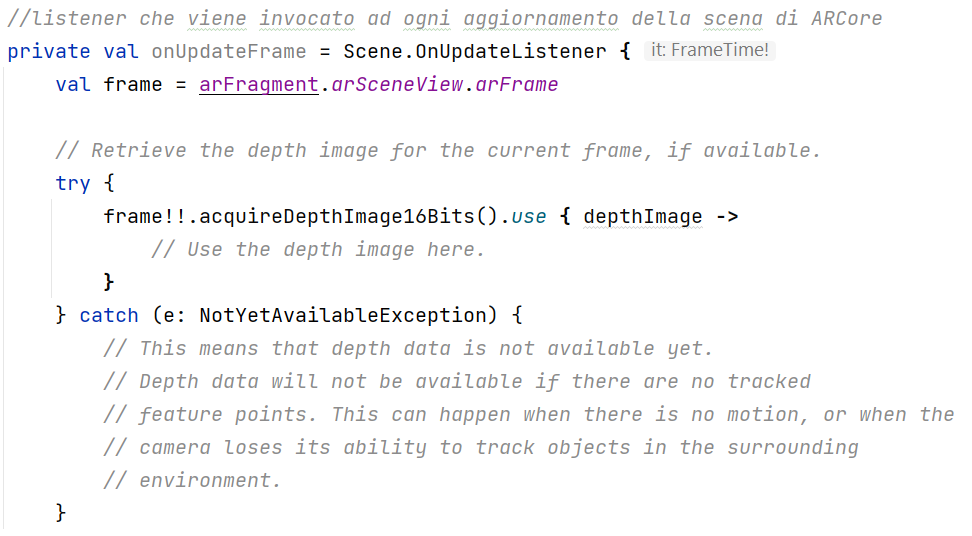
\includegraphics[width=0.8\textwidth]{../../resources/images/depthAPI/depthAPI2.PNG}}%
			{Fonte: \url{https://developers.google.com/ar/develop/java/depth/developer-guide}}
			\caption{Immagine di profondità}
			\label{fig: Immagine di profondità}
		\end{figure}
		
		\section{Depth Hit Test}
		
		Hit Test sono sono stati una fondamentale interazione per le applicazioni di realtà aumentata e permettono agli utenti 			di posizionare oggetti 3d in una posizione precisa in una scena. Solitamente queste azioni potevano essere eseguite su 			superfici piane. Integrando la profondità sono stati ottenuti degli hit test più precisi grazie ai quali è possibile  			posizionare contenuti virtuali anche su superfici non piane in aree con bassa texture. (Esempio \vref{fig: Depth Hit Test})\\

		\begin{figure}
			\centering
			\copyrightbox[0.5]{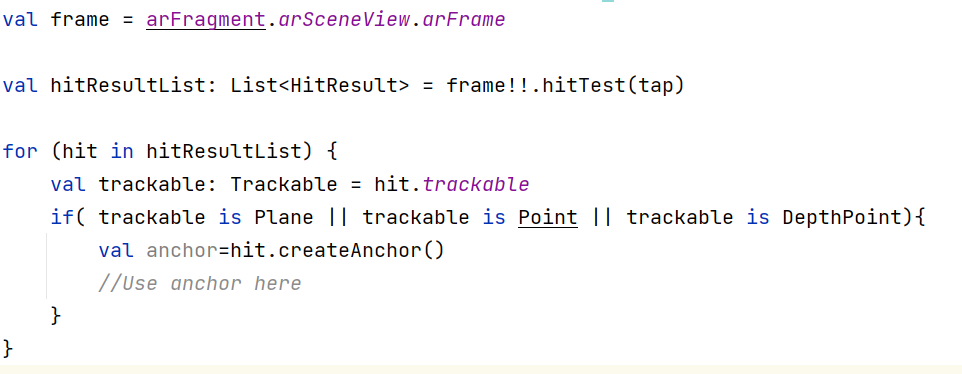
\includegraphics[width=0.8\textwidth]{../../resources/images/depthAPI/depthAPI3.PNG}}%
			{Fonte: \url{https://developers.google.com/ar/develop/java/depth/developer-guide}}
			\caption{Depth Hit Test}
			\label{fig: Depth Hit Test}
		\end{figure}
\end{document}
	\documentclass[crop=false, class=book]{standalone}

%impostazioni lingua
\usepackage[T1]{fontenc}
\usepackage[utf8]{inputenc}
\usepackage[english,italian]{babel}

\usepackage[dvipsnames]{xcolor}
\usepackage{listings}

\lstdefinelanguage{Kotlin}{
	comment=[l]{//},
	commentstyle={\color{gray}\ttfamily},
	emph={[1]first, firstOrNull, forEach, lazy, map, mapNotNull, println},
	emphstyle={[1]\color{OrangeRed}},
	identifierstyle=\color{black},
	keywords={!in, !is, abstract, actual, annotation, as, as?, break, by, catch, class, companion, const, constructor, continue, crossinline, data, delegate, do, dynamic, else, enum, expect, external, false, field, file, final, finally, for, fun, get, if, import, in, infix, init, inline, inner, interface, internal, is, lateinit, noinline, null, object, open, operator, out, override, package, param, private, property, protected, public, receiveris, reified, return, return@, sealed, set, setparam, super, suspend, tailrec, this, throw, true, try, typealias, typeof, val, var, vararg, when, where, while, it},
	keywordstyle={\color{NavyBlue}\bfseries},
	morecomment=[s]{/*}{*/},
	morestring=[b]",
	morestring=[s]{"""*}{*"""},
	ndkeywords={@Deprecated, @JvmField, @JvmName, @JvmOverloads, @JvmStatic, @JvmSynthetic, Array, Byte, Double, Float, Int, Integer, Iterable, Long, Runnable, Short, String, Any, Unit, Nothing, Config, LightEstimationMode, CameraConfigFilter, CameraConfig, FacingDirection, AugmentedFaceMode, AugmentedFace, TrackingState, RegionType, CloudAnchorMode,AugmentedImageDatabase, BitmapFactory, Session, InstantPlacementMode, File, Uri, RecordingConfig },
	ndkeywordstyle={\color{BurntOrange}\bfseries},
	sensitive=true,
	stringstyle={\color{ForestGreen}\ttfamily},
	emph={[2]FRONT,MESH3D,ENVIRONMENTAL\_HDR,AMBIENT\_INTENSITY, DISABLED,FOREHEAD\_LEFT,FOREHEAD\_RIGHT,NOSE\_TIP, TRACKING, ENABLED, LOCAL\_Y\_UP},
	emphstyle={[2]\color{Purple}\ttfamily},
}

\definecolor{lightgrey}{RGB}{230,237,244}

\lstset{
	basicstyle=\scriptsize\sffamily\color{black},
	backgroundcolor=\color{lightgrey},
	frame=single,
	numbers=left,
	numbersep=5pt,
	numberstyle=\tiny\color{gray},
	showspaces=false,
	showstringspaces=false,
	tabsize=1,
	texcl=true,
	captionpos=b,
	breaklines=true
}




%sistema i margini
\usepackage{geometry}
\geometry{a4paper,top=2.2cm,bottom=2.2cm,left=3cm,right=3cm, heightrounded}

%interlinea 1.5
\usepackage{setspace}
\onehalfspacing

%gestione delle testatine
\usepackage{fancyhdr}
\pagestyle{fancy}
\lhead{}
\chead{}
\rhead{Titolo}
\lfoot{}
\cfoot{\thepage}
\rfoot{}
\renewcommand{\headrulewidth}{0.4pt}

%formattazione titoli paragrafo
\usepackage{titlesec}
\titleformat{\chapter}[block]{\normalfont\huge\bfseries}{\thechapter.}{0.7em}{\huge}

%pacchetti per i riferimenti in bibliografia
\usepackage[autostyle,italian=guillemets]{csquotes}
\usepackage[style=numeric,citestyle=numeric-comp,backend=biber]{biblatex}

%risorsa che contiene la bibliografia
\addbibresource{./../bibliografia.bib}

\usepackage{lipsum}
\usepackage{graphicx}
\usepackage[italian]{varioref}
\usepackage{copyrightbox}



\begin{document}

	\chapter{User Interaction}
	ARCore utilizza la tecnologia \textit{ray casting} per permettere all'utente di posizionare un oggetto nella scena corrente 	in un punto fissato. Quando lo schermo del telefono viene toccato o viene compiuta qualche altra interazione, 					viene proiettato un raggio nella visuale del mondo della fotocamera che può intersecare un preciso punto o piani geometrici. ARCore permette di ricavare un elenco dei risultati delle intersezioni con la geometria della scena rilevata attraverso gli hitTest. Solitamente il primo risultato è quello più significativo perchè si riferisce all'intersezione più vicina al dispositivo.\\
			
	
\end{document}
	\documentclass[crop=false, class=book]{standalone}

\usepackage{graphicx}
\usepackage[italian]{varioref}
\usepackage{copyrightbox}
\usepackage{listings}
\usepackage{subfig}

\begin{document}
		
	\chapter{Oriented Points}
	
		ARCore utilizza i punti orientati quando vengono toccate superfici che non sono piane (figura~\vref{fig: surf-arb}). Attorno al punto individuato dal tocco vengono esaminati dei punti caratteristici grazie ai quali è possibile stimare l'angolo dell'intersezione \cite{anna2018arcoredetection}. Il punto orientato è costituito dal risultato del hitTest che prende in considerazione questo angolo. 
		L'invocazione del metodo \verb|getOrientationMode()| su un oggetto Point consente di ritornare l'enumerazione \verb|Point.OrientationMode| che restituisce la \textbf{modalità di orientamento} del punto.\\
		La modalità di orientamento può essere di due tipi:
		\begin{itemize}
			\item \textit{ESTIMATED SURFACE NORMAL} se la coordinata X è perpendicolare al raggio di proiezione e parallela alla superficie fisica centrata attorno al hitTest; Y giace sulla normale alla superficie stimata e Z punta verso la direzione dell'utente.
			\item \emph{INITIALIZED TO IDENTITY} l'orientamento è inizializzato in base all'identità (unitario) ma può variare con il tempo. Ciò che cambia dall'altra modalità è che la coordinata X punta verso la prospettiva del dispositivo dell'utente, ed Y punta verso l'alto.
		\end{itemize}
		
				
		\begin{figure}[h]
				\centering
				\copyrightbox[b]{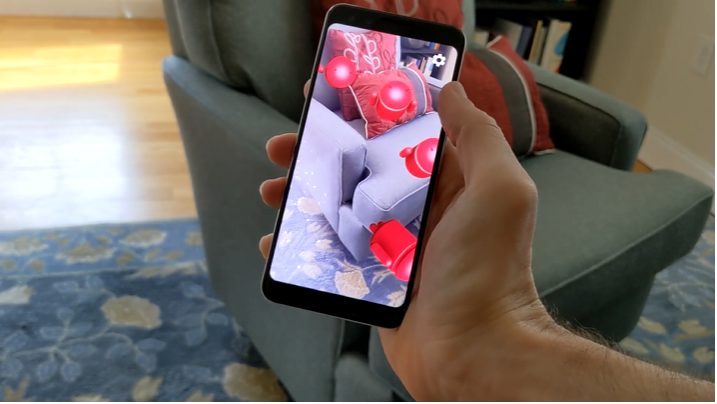
\includegraphics[width=0.8\textwidth]{./resources/images/OrientedPoints/points1.png}}%
				{Fonte: \url{https://developers.google.com/ar/develop/java/depth/developer-guide}}
				\caption{Esempio di punti orientati su una superficie arbitraria}
				\label{fig: surf-arb}
		\end{figure}
		
		
\end{document}
	\documentclass[crop=false, class=book]{standalone}

\usepackage{graphicx}
\usepackage[italian]{varioref}
\usepackage{copyrightbox}

\begin{document}

	\chapter{HitTest}
	
	Un \textit{HitTest} è il risultato che viene restituito quando viene toccato un determinato oggetto \verb|Trackable|.
	Ogni risultato è costituito da:
	\begin{itemize}
		\item \textbf{Lunghezza in metri} dall'origine del raggio che può essere ricavata dall'invocazione del metodo \verb|getDistance()|.
		\item \textbf{Posa} (posizione e orientamento) del punto toccato con \verb|getHitPose()|.
		\item \textbf{Istanza Trackable} che contiene la geometria 3d che è stata toccata con \verb|getTrackable()|.
	\end{itemize}
	
	\noindent
	Questo risultato può essere utilizzato per definire un'ancora che permette di fissare la posizione di contenuti virtuali all'interno dello spazio. L'ancora si adatta agli aggiornamenti dell'ambiente circostante e aggiorna gli oggetti legati ad essa come descritto nel capitolo~\vref{cap:anchor} relativo ad Anchor e Trackable.\\
	
	\noindent
	Esistono quattro tipi di risultati che si possono ottenere in una sessione ARCore:
		\begin{itemize}
		\item \textbf{Profondità}: richiede l'attivazione di depth API nella sessione ARCore ed è usato per posizionare oggetti su superfici arbitrarie (non solo su piani).
		\item \textbf{Aereo}: permette di posizionare un oggetto su superfici piane e utilizza la loro geometria per determinare la profondità e l'orientamento del punto individuato.
		\item \textbf{Punto caratteristico}: permette di disporre oggetti in superfici arbitrarie basandosi su caratteristiche visive attorno al punto sul quale l'utente tocca. 
		\item \textbf{Posizionamento istantaneo}: consente di posizionare un oggetto rapidamente in un piano utilizzando la sua geometria completa attorno al punto selezionato. 
	\end{itemize}
	\clearpage
	
	\section{Definizione e gestione di un HitTest}
	E' possibile ricevere un \verb|HitTest| di tipo diverso come descritto dal listing~\vref{lst: hitTest-filter}.
	\begin{center}
		\begin{minipage}{0.95\textwidth}
			\begin{lstlisting}[caption={Filtraggio hitTest in base al tipo.}, label={lst: hitTest-filter}, language=Kotlin]
			// I risultati dell'hit-test sono ordinati per distanza crescente dalla fotocamera.
			val hitResultList =
  				if (usingInstantPlacement) {
    				// Se si usa la modalità Instant Placement, il valore in 
    				// APPROXIMATE DISTANCE METERS determina quanto lontano sarà 
    				// piazzato l'anchor, dal punto di vista della fotocamera.
    				frame.hitTestInstantPlacement(tap.x, tap.y, APPROXIMATE_DISTANCE_METERS)
    				// I risultati dell'Hit-test usando Instant Placement 
    				// avranno un solo risultato di tipo InstantPlacementResult.
  				} else {
    				frame.hitTest(tap)
  				}
  				
			// Il primo hit result di solito è il più rilevante per rispondere agli input dell'utente.
			val firstHitResult = hitResultList.firstOrNull { hit ->
  					val trackable = hit.trackable!!
  					
  					if(trackable is DepthPoint){
  						// Sostituisci con un qualsiasi oggetto Trackable
  						true
  					} else {
  						false
  					}
  				}
  				
			if (firstHitResult != null) {
  				// Utilizza l'hit result. Ad esempio crea un anchor su tale punto di interesse.
  				val anchor = firstHitResult.createAnchor()
  				// Utilizzo dell'anchor...
			}
			\end{lstlisting}
		\end{minipage}
	\end{center}
	
	
	\noindent
	Per definire un hitTest attraverso un raggio \textbf{arbitrario} si può usare il metodo \verb|Frame.hitTest(origin3: Array<float>, originOffset: int, direction3:| \\
	\verb|Array<float>, originOffset: int)| dove i quattro parametri specificano:
	
	\begin{itemize}
		\item \verb|origin3|: array che contiene le 3 coordinate del punto di partenza del raggio.
		\item \verb|originOffset|: offset sommato alle coordinate dell'array di partenza.
		\item \verb|director3|: array che contiene le 3 coordinate del punto di arrivo del raggio.
		\item \verb|directorOffset|: offset sommato alle coordinate dell'array di arrivo.
	\end{itemize}
	
	\noindent
	
	Per creare un anchor sul risultato del tocco viene usato \verb|hitResult.createAnchor()| che restituirà un anchor disposto 		sul \verb|Trackable| sottostante su cui è avvenuto il tocco.
	Nel caso della nostra applicazione il risultato restituito da hitTest nella modalità \emph{Plane Detection} è di tipo 			\verb|Aereo|; il rilevamento di un piano consente di disporre un animale in un punto preciso. Questo evento è stato gestito 	dal metodo \verb|setOnTapArPlaneListener| riportato nell'esempio di codice \vref{lst: Definizione Anchor in Plane 				Detection}.\\
	Oltre all'oggetto hitTest è stato molto importante \verb|hitTestResult| definito nella documentazione di 						\emph{sceneView}. Questo oggetto mantiene tutti gli hitTest che vengono creati quando l'utente tocca lo schermo. 				Inoltre, contiene le informazioni associate al nodo che è stato colpito dal hitTest. Quando l'utente posiziona un'animale 		in 	un piano, viene creato un oggetto \verb|anchorNode| passando al costruttore l'anchor generato dal 							hitTest. Successivamente, viene aggiunto un oggetto \verb|TransformableNode| come nodo figlio di AnchorNode. Questo 			tipo di nodo può essere utilizzato per aggiungere un oggetto \verbe|Node| come figlio, per eseguire operazioni di 				traslazione, selezione, rotazione e scala. L'utilizzo di hitTestResult è stato utile nell'eliminazione degli animali perchè 	ci ha dato la possibilità di ricavare l'oggetto Node associato all'animale che l'utente voleva eliminare. Per rilevare un 		hitTestResult viene invocato il metodo setOnTouchListener(delNode) su TransformableNode dove delNode è un oggetto di tipo 		Node.OnTouchListener.\\	Nell'esempio \vref{lst: delete-node} è riportato il codice dell'eliminazione di un nodo dalla 			scena.
	
	\begin{center}
		\begin{minipage}{0.95\textwidth}
			\begin{lstlisting}[caption={Eliminazione di un nodo dalla scena in Plane Detection}, label={lst: delete-node}, language=Kotlin]
			//Listener per eliminare i nodi
        	val delNode =
            	Node.OnTouchListener { hitTestResult, motionEvent ->
                	if(switchButton.isChecked){
                    	Log.d(TAG, "handleOnTouch")

                    	// Prima chiamata ad ArFragment per gestire TrasformableNode
                    	arFragment.onPeekTouch(hitTestResult, motionEvent)

                    	//La rimozione si verifica con un evento ACTION_UP
                    	if (motionEvent.action == MotionEvent.ACTION_UP) {

                        	if (hitTestResult.node != null && switchButton.isChecked) {

                            	Log.d(TAG, "handleOnTouch hitTestResult.getNode() != null")

                            	//Restituisce il nodo che è stato colpito dal hitTest
                            	val hitNode: Node? = hitTestResult.node

                            	hitNode!!.renderable = null

                            	hitNode.parent = null

                            	//Eliminazione di tutti i figli del nodo
                            	val children =hitNode.children
                            	if(children.isNotEmpty() && children != null){
                                	for (i in 0 until children.size){
                                    children[i].renderable = null
                                	}
                            	}

                            	arFragment.arSceneView.scene.removeChild(hitNode)
                        	}
                    	}
                	}
                true
            }
			\end{lstlisting}
		\end{minipage}
	\end{center}
	
			
	
\end{document}
	\documentclass[crop=false, class=book]{standalone}

%impostazioni lingua
\usepackage[T1]{fontenc}
\usepackage[utf8]{inputenc}
\usepackage[english,italian]{babel}

\usepackage[dvipsnames]{xcolor}
\usepackage{listings}

\lstdefinelanguage{Kotlin}{
	comment=[l]{//},
	commentstyle={\color{gray}\ttfamily},
	emph={[1]first, firstOrNull, forEach, lazy, map, mapNotNull, println},
	emphstyle={[1]\color{OrangeRed}},
	identifierstyle=\color{black},
	keywords={!in, !is, abstract, actual, annotation, as, as?, break, by, catch, class, companion, const, constructor, continue, crossinline, data, delegate, do, dynamic, else, enum, expect, external, false, field, file, final, finally, for, fun, get, if, import, in, infix, init, inline, inner, interface, internal, is, lateinit, noinline, null, object, open, operator, out, override, package, param, private, property, protected, public, receiveris, reified, return, return@, sealed, set, setparam, super, suspend, tailrec, this, throw, true, try, typealias, typeof, val, var, vararg, when, where, while, it},
	keywordstyle={\color{NavyBlue}\bfseries},
	morecomment=[s]{/*}{*/},
	morestring=[b]",
	morestring=[s]{"""*}{*"""},
	ndkeywords={@Deprecated, @JvmField, @JvmName, @JvmOverloads, @JvmStatic, @JvmSynthetic, Array, Byte, Double, Float, Int, Integer, Iterable, Long, Runnable, Short, String, Any, Unit, Nothing, Config, LightEstimationMode, CameraConfigFilter, CameraConfig, FacingDirection, AugmentedFaceMode, AugmentedFace, TrackingState, RegionType, CloudAnchorMode,AugmentedImageDatabase, BitmapFactory, Session, InstantPlacementMode, File, Uri, RecordingConfig },
	ndkeywordstyle={\color{BurntOrange}\bfseries},
	sensitive=true,
	stringstyle={\color{ForestGreen}\ttfamily},
	emph={[2]FRONT,MESH3D,ENVIRONMENTAL\_HDR,AMBIENT\_INTENSITY, DISABLED,FOREHEAD\_LEFT,FOREHEAD\_RIGHT,NOSE\_TIP, TRACKING, ENABLED, LOCAL\_Y\_UP},
	emphstyle={[2]\color{Purple}\ttfamily},
}

\definecolor{lightgrey}{RGB}{230,237,244}

\lstset{
	basicstyle=\scriptsize\sffamily\color{black},
	backgroundcolor=\color{lightgrey},
	frame=single,
	numbers=left,
	numbersep=5pt,
	numberstyle=\tiny\color{gray},
	showspaces=false,
	showstringspaces=false,
	tabsize=1,
	texcl=true,
	captionpos=b,
	breaklines=true
}




%sistema i margini
\usepackage{geometry}
\geometry{a4paper,top=2.2cm,bottom=2.2cm,left=3cm,right=3cm, heightrounded}

%interlinea 1.5
\usepackage{setspace}
\onehalfspacing

%gestione delle testatine
\usepackage{fancyhdr}
\pagestyle{fancy}
\lhead{}
\chead{}
\rhead{Titolo}
\lfoot{}
\cfoot{\thepage}
\rfoot{}
\renewcommand{\headrulewidth}{0.4pt}

%formattazione titoli paragrafo
\usepackage{titlesec}
\titleformat{\chapter}[block]{\normalfont\huge\bfseries}{\thechapter.}{0.7em}{\huge}

%pacchetti per i riferimenti in bibliografia
\usepackage[autostyle,italian=guillemets]{csquotes}
\usepackage[style=numeric,citestyle=numeric-comp,backend=biber]{biblatex}

%risorsa che contiene la bibliografia
\addbibresource{./../bibliografia.bib}

\usepackage{lipsum}
\usepackage{graphicx}
\usepackage[italian]{varioref}
\usepackage{copyrightbox}
\usepackage{subfig}

\begin{document}
		
	\chapter{Anchor and Trackable}
	
		ARCore definisce gli Anchor per assicurare che gli oggetti virtuali rimangano nella stessa posizione e vengano 					tracciati nel tempo. L'ambiente circostante può cambiare, ed è necessario che la posizione di questi oggetti
		rimanga stabile. Gli Anchor sono disposti in insieme di punti o piani rappresentati da oggetti di tipo Trackable.\\
		Gli oggetti Trackable rappresentano la forma geometrica sulla quale verranno definiti gli anchor.
		Su questi oggetti possono essere invocati 3 metodi:
		\begin{itemize}
			\item[•] \emph{createAnchor(pose: Pose)} crea un anchor in una posa che è definita nel Trackable corrente. Il tipo di oggetto Trackable definirà il modo con cui l'anchor verrà disposto e la modalità di aggiornamento della sua posa mentre il modello del mondo varia.
			\item[•] \emph{ getAnchors()} restituisce tutti gli anchor presenti nel dato Trackable.
			\item[•] \emph{getTrackingState()} restituisce un oggetto TrackingState che rappresenta lo stato del Trackable. Questo stato può essere: PAUSED quando il rilevamento viene perso ma potrebbe riprendere in futuro; STOPPED quando viene fermato e non verrà più ripreso; TRACKING se viene tracciato il determinato Trackable.
		\end{itemize}
		\begin{flushleft}
			La definizione di anchor e lo stato di tracciamento sono stati molto importanti per la definizione delle 						funzionalità principali della nostra applicazione.\\
	 		In base alla modalità l'applicazione offre funzionalità differenti:
		\end{flushleft}
	 	\begin{itemize}
	 		\item \emph{Plane Detection}: ARCore rileva dei piani (Trackable) sui quali è possibile posizionare degli animali virtuali. In particolare, quando l'utente tocca un punto preciso del piano viene definito un anchor sul quale verrà renderizzato il modello 3d dell'animale. (Codice in \vref{lst: Definizione Anchor in Plane Detection})
	 	
	 		\item \emph{Augmented Images}: in ciascun frame viene controllato se lo stato di un'immagine aumentata è TRACKING; in questo caso l'immagine viene riconosciuta e viene definito un anchor nel suo centro nel quale verrà renderizzato il modello del pianeta corrispondente. (Codice in \vref{lst: Definizione Anchor in Augmented Images})
	 	\end{itemize}
		
		\clearpage
		\begin{center}
				\begin{minipage}{1.1\textwidth}
					\begin{lstlisting}[caption={Definizione Anchor in Plane Detection}, label={lst: Definizione Anchor in Plane Detection}, language=Kotlin]
					 //Evento che si verifica quando viene toccato un piano
            		 arFragment.setOnTapArPlaneListener { hitResult, plane, motionEvent ->

                	 //Se siamo nella modalità place model
                	 if (!switchButton.isChecked) {

                     arFragment.arSceneView.scene.addChild(AnchorNode(hitResult.createAnchor()).apply {
 
                        // Crea il transformable model e lo aggiunge all'anchor
                        addChild(TransformableNode(arFragment.transformationSystem).apply {

                            setModel()
                            renderable = objRenderable
                            
                            //...
					
						\end{lstlisting}
					\end{minipage}
		\end{center}
		\vspace{0.2cm}
		\begin{center}
			\begin{minipage}{1.1\textwidth}
				\begin{lstlisting}[caption={Definizione Anchor in Augmented Images}, label={lst: Definizione Anchor in Augmented Images}, 	language=Kotlin]
				//Per ogni immagine tracciata  se non è presente il  modello allora viene immediatamente costruito e instanziato
        		for (augmentedImage in augmentedImages) {

            		if (augmentedImage.trackingState == TrackingState.TRACKING) {

                		for (i in 0 until namesobj.size) {

                    		if (augmentedImage.name.contains(namesobj[i]) && !renderobj[i]) {

                        		Toast.makeText(this,""+namesobj[i]+" rilevato",Toast.LENGTH_SHORT).show()

                        		if(namesobj[i]=="systemsolar"){
                            		renderObject(
                                		arFragment,
                                		augmentedImage.createAnchor(augmentedImage.centerPose),
                                		"solar_system"
                            		)
                        		}else {
                            		renderObject(
                                		arFragment,
                                		augmentedImage.createAnchor(augmentedImage.centerPose),
                                		namesobj[i]
                            		)
                        		}	
                        		renderobj[i] = true
                    		}
                		}
            		}
        		}
					\end{lstlisting}
			\end{minipage}
		\end{center}
	
		\clearpage
		
		\begin{flushleft}
			Di seguito è riportata una rappresentazione di come un oggetto virtuale viene disposto in un piano.
		\end{flushleft}
		\begin{figure}
				\centering
				\copyrightbox[0.5]{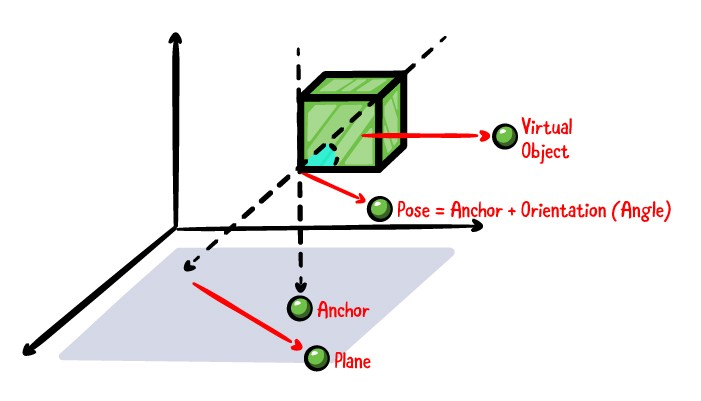
\includegraphics[width=0.7\textwidth]{../../resources/images/UserInteraction/Anchor.jpeg}}%
				{Fonte: \url{https://medium.com/@jaaveeth.developer/arcore-81528569eb2c}}
				\caption{Oggetto virtuale in un piano}
				\label{fig: Oggetto virtuale in un piano}
		\end{figure}	

	\begin{flushleft}
		Nella modalità \emph{Plane Detection} la posa (posizione e orientamento) di un animale rimane invariata anche se 				l'ambiente circostante cambia.\\
		Qui sotto sono riportati degli esempi in cui si può notare che il pinguino rimane nello stesso punto da qualsiasi 				prospettiva e distanza.
	\end{flushleft}
	
	\begin{figure}
			\centering
			\copyrightbox[b]{
				\subfloat[][\emph{Pinguino da un'inquadratura vicina}]
				{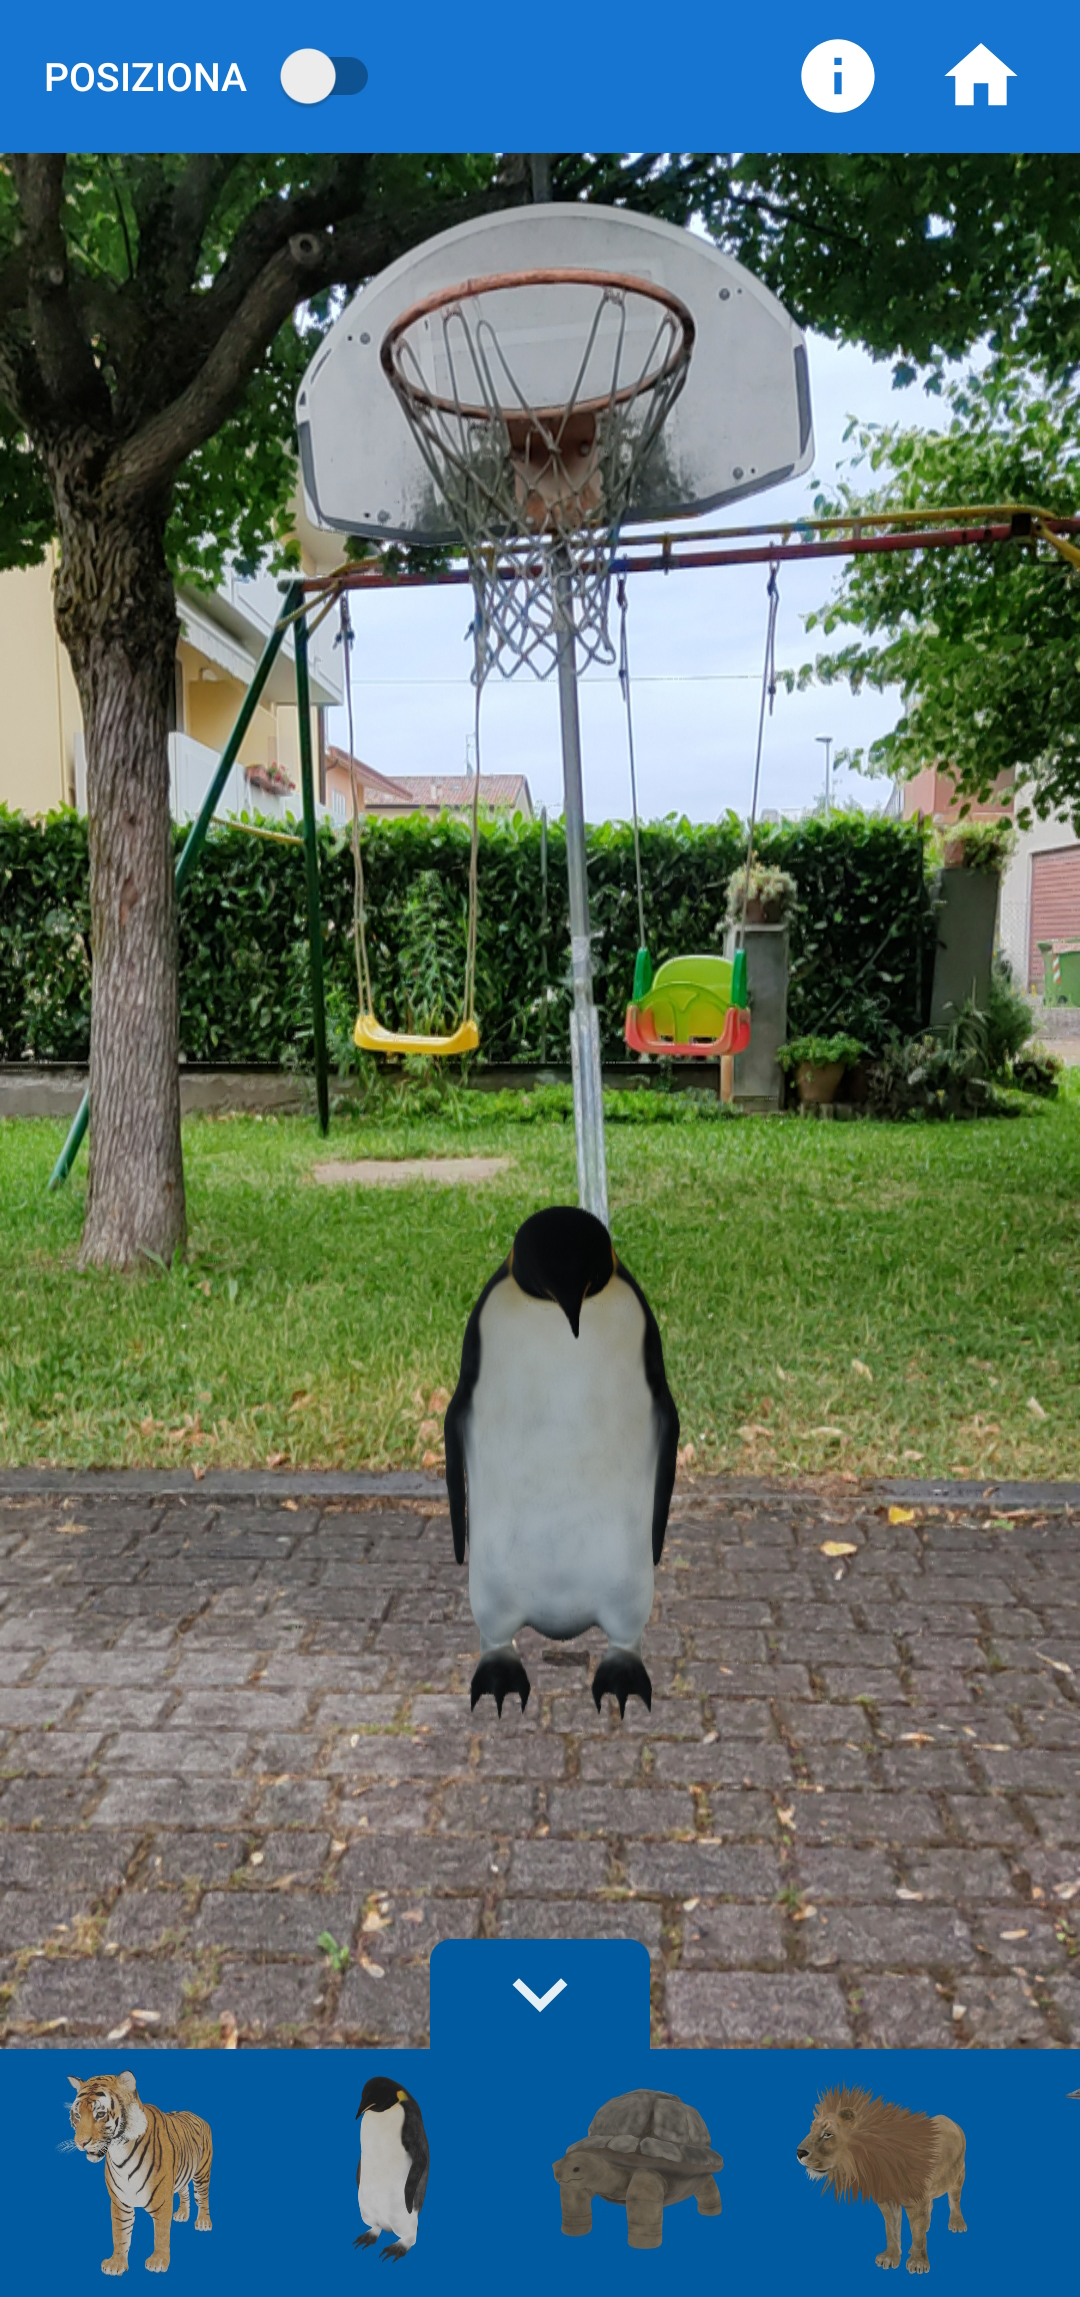
\includegraphics[width=0.28\textwidth]{../../resources/images/AnchorTrackable/pingvicino.jpg}}  \quad,
				\subfloat[][\emph{Pinguino da un'inquadratura lontana}]
				{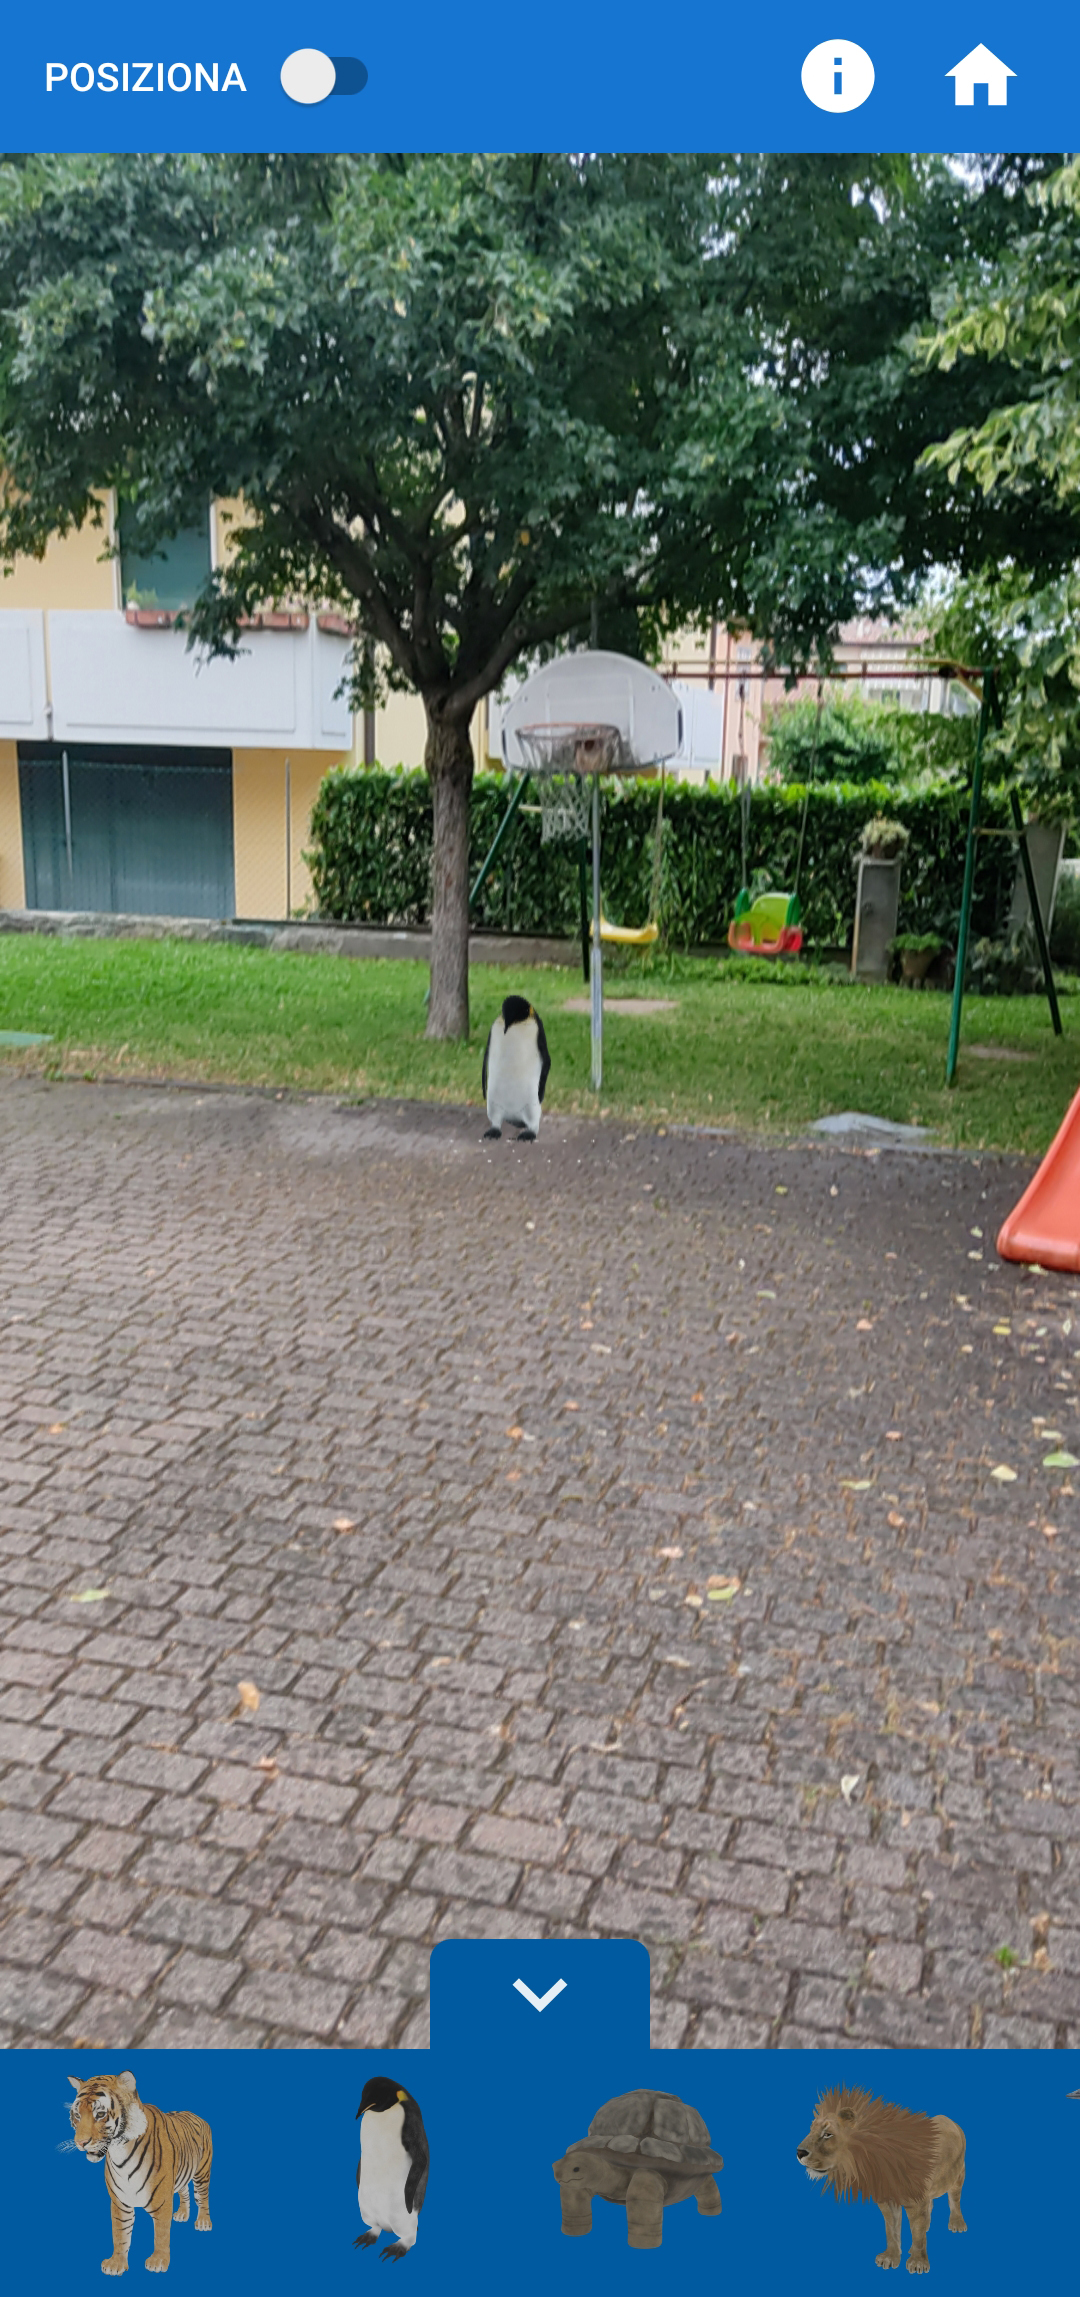
\includegraphics[width=0.28\textwidth]{../../resources/images/AnchorTrackable/pinglontano1.jpg}} \quad,
				\subfloat[][\emph{Giove da lontano}]
				{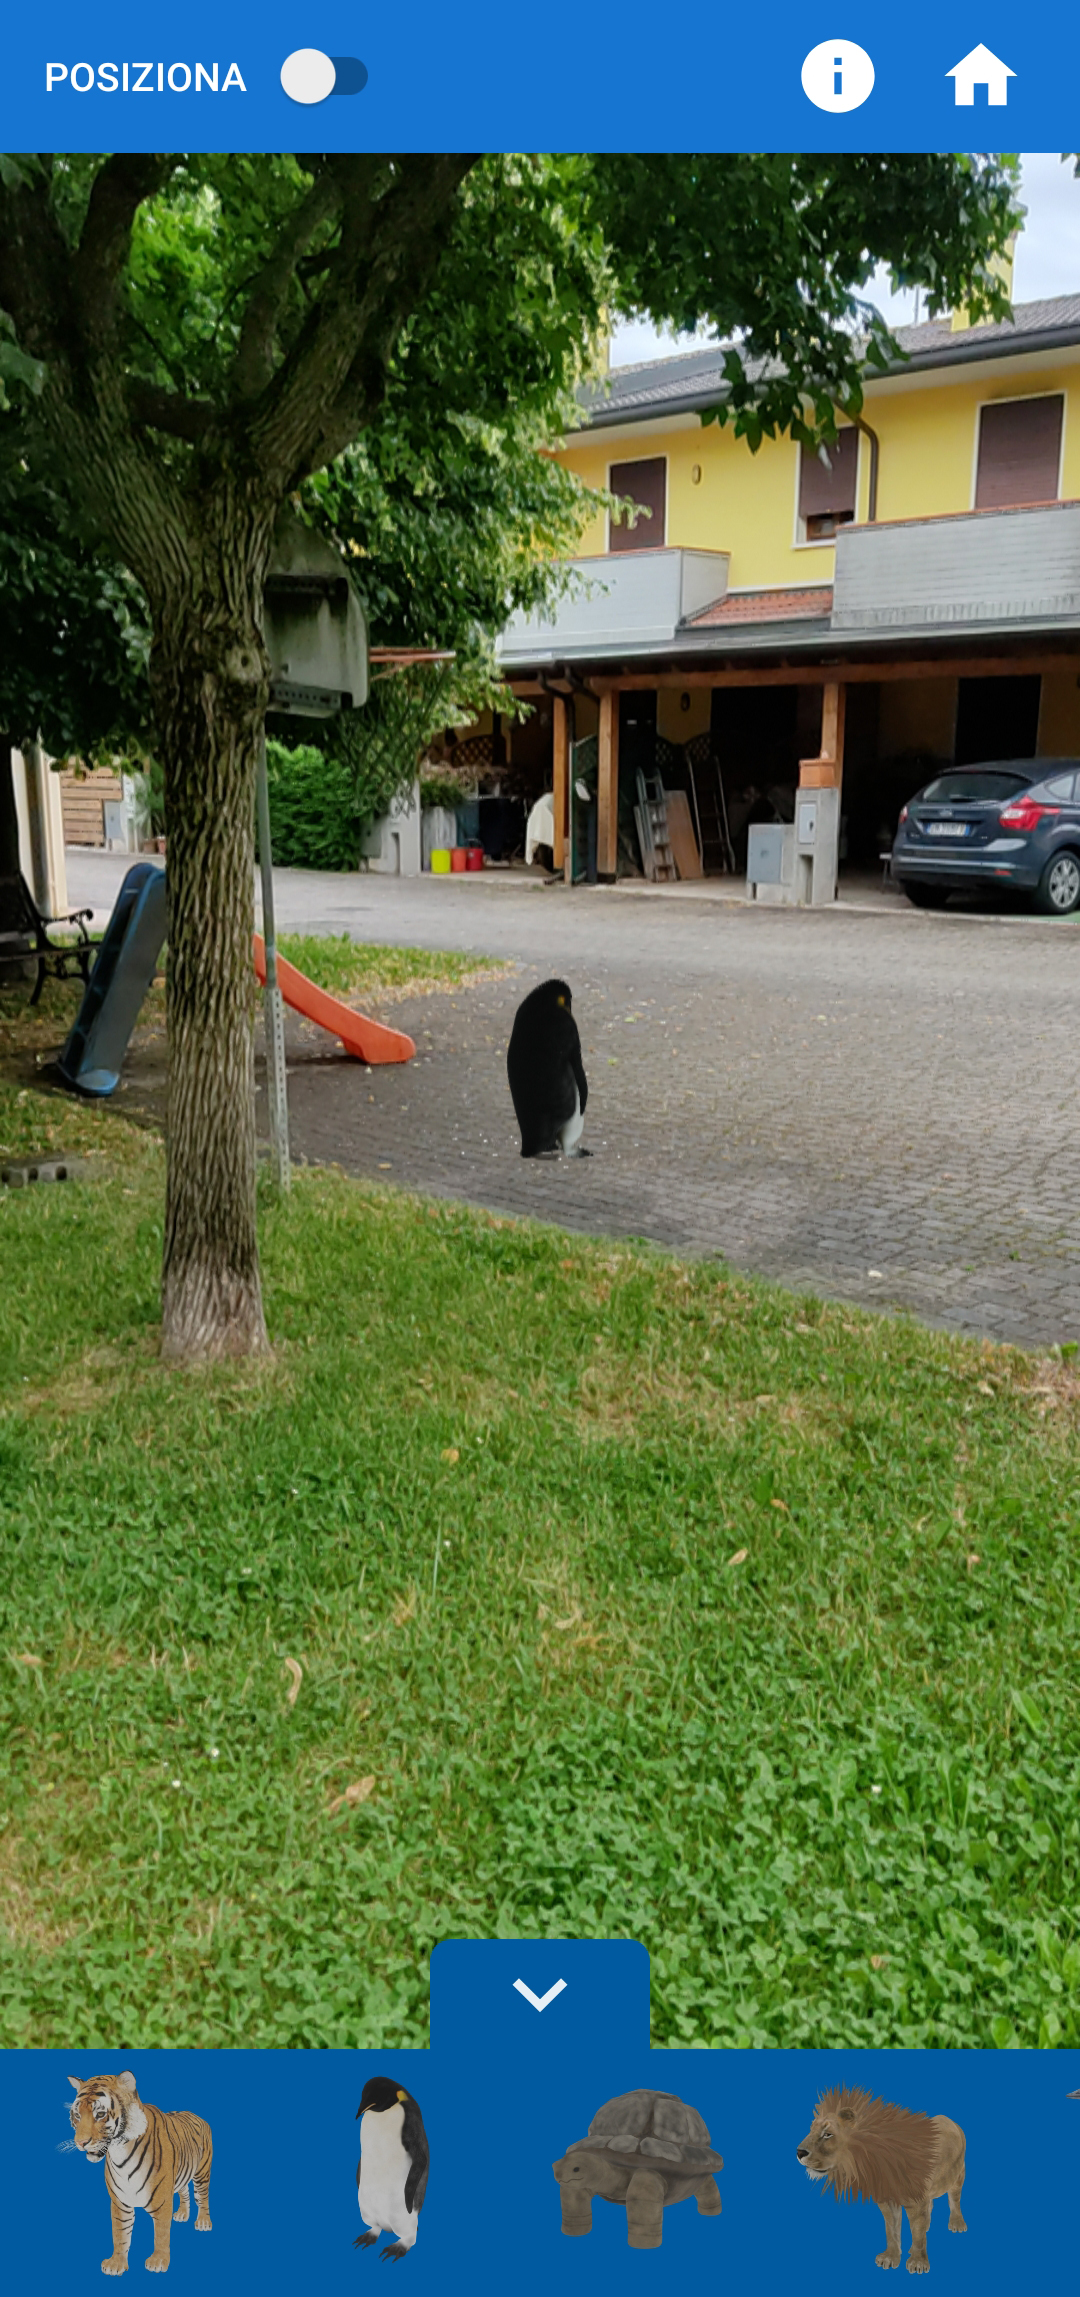
\includegraphics[width=0.28\textwidth]{../../resources/images/AnchorTrackable/pinglontano2.jpg}}
			}{Fonte: \url{https://developers.google.com/}}	
			\caption{Esempio di inquadrature differenti in Plane Detection}
			\label{fig:augm_img}
	\end{figure}	
	
		
	\begin{figure}
			\centering
			\copyrightbox[b]{
				\subfloat[][\emph{Tracciamento immagine}]
				{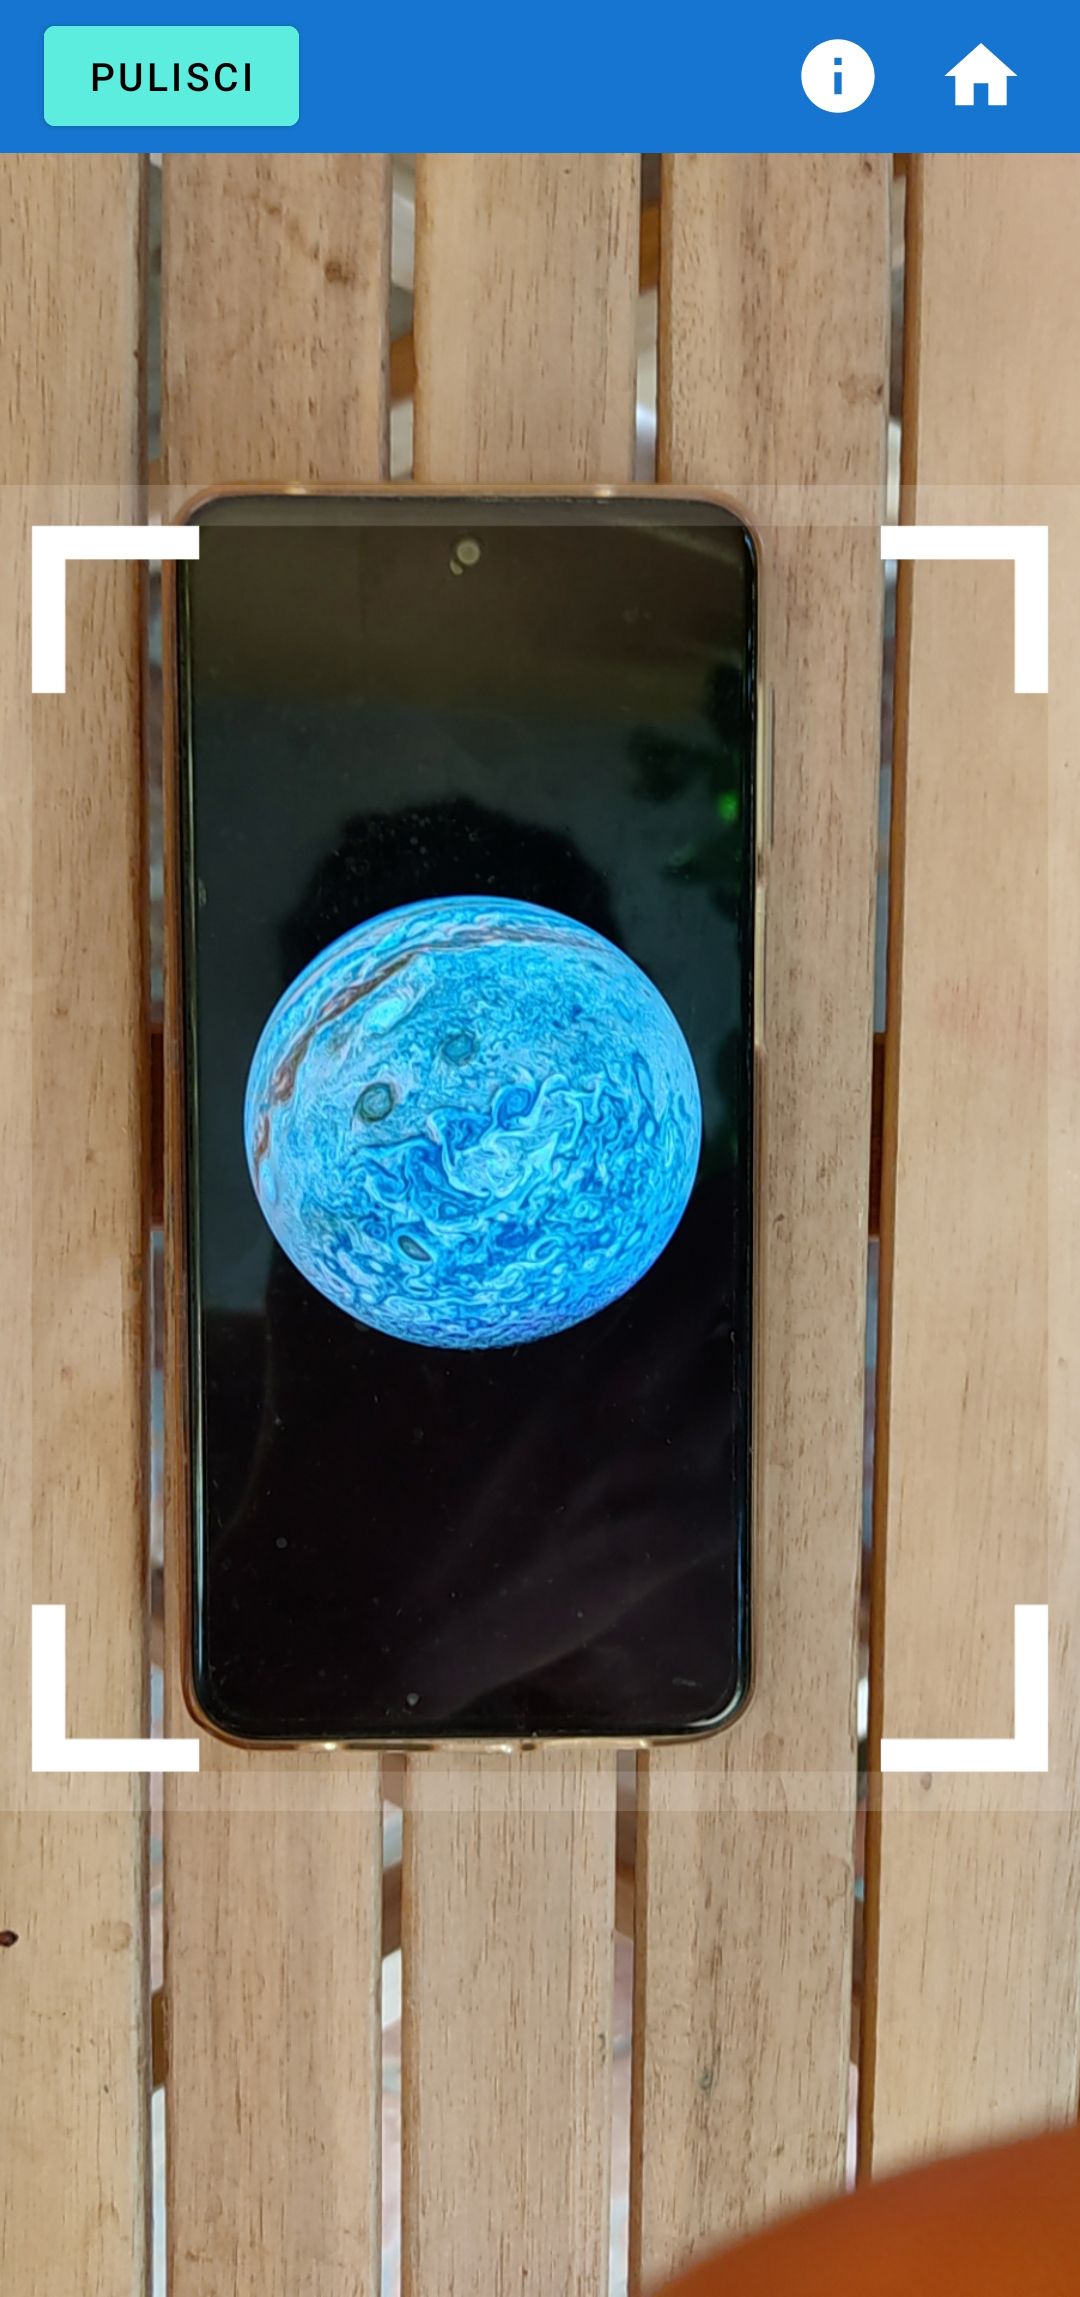
\includegraphics[width=0.28\textwidth]{../../resources/images/AnchorTrackable/Giove2d.jpg}}  \,
				\subfloat[][\emph{Giove da vicino}]
				{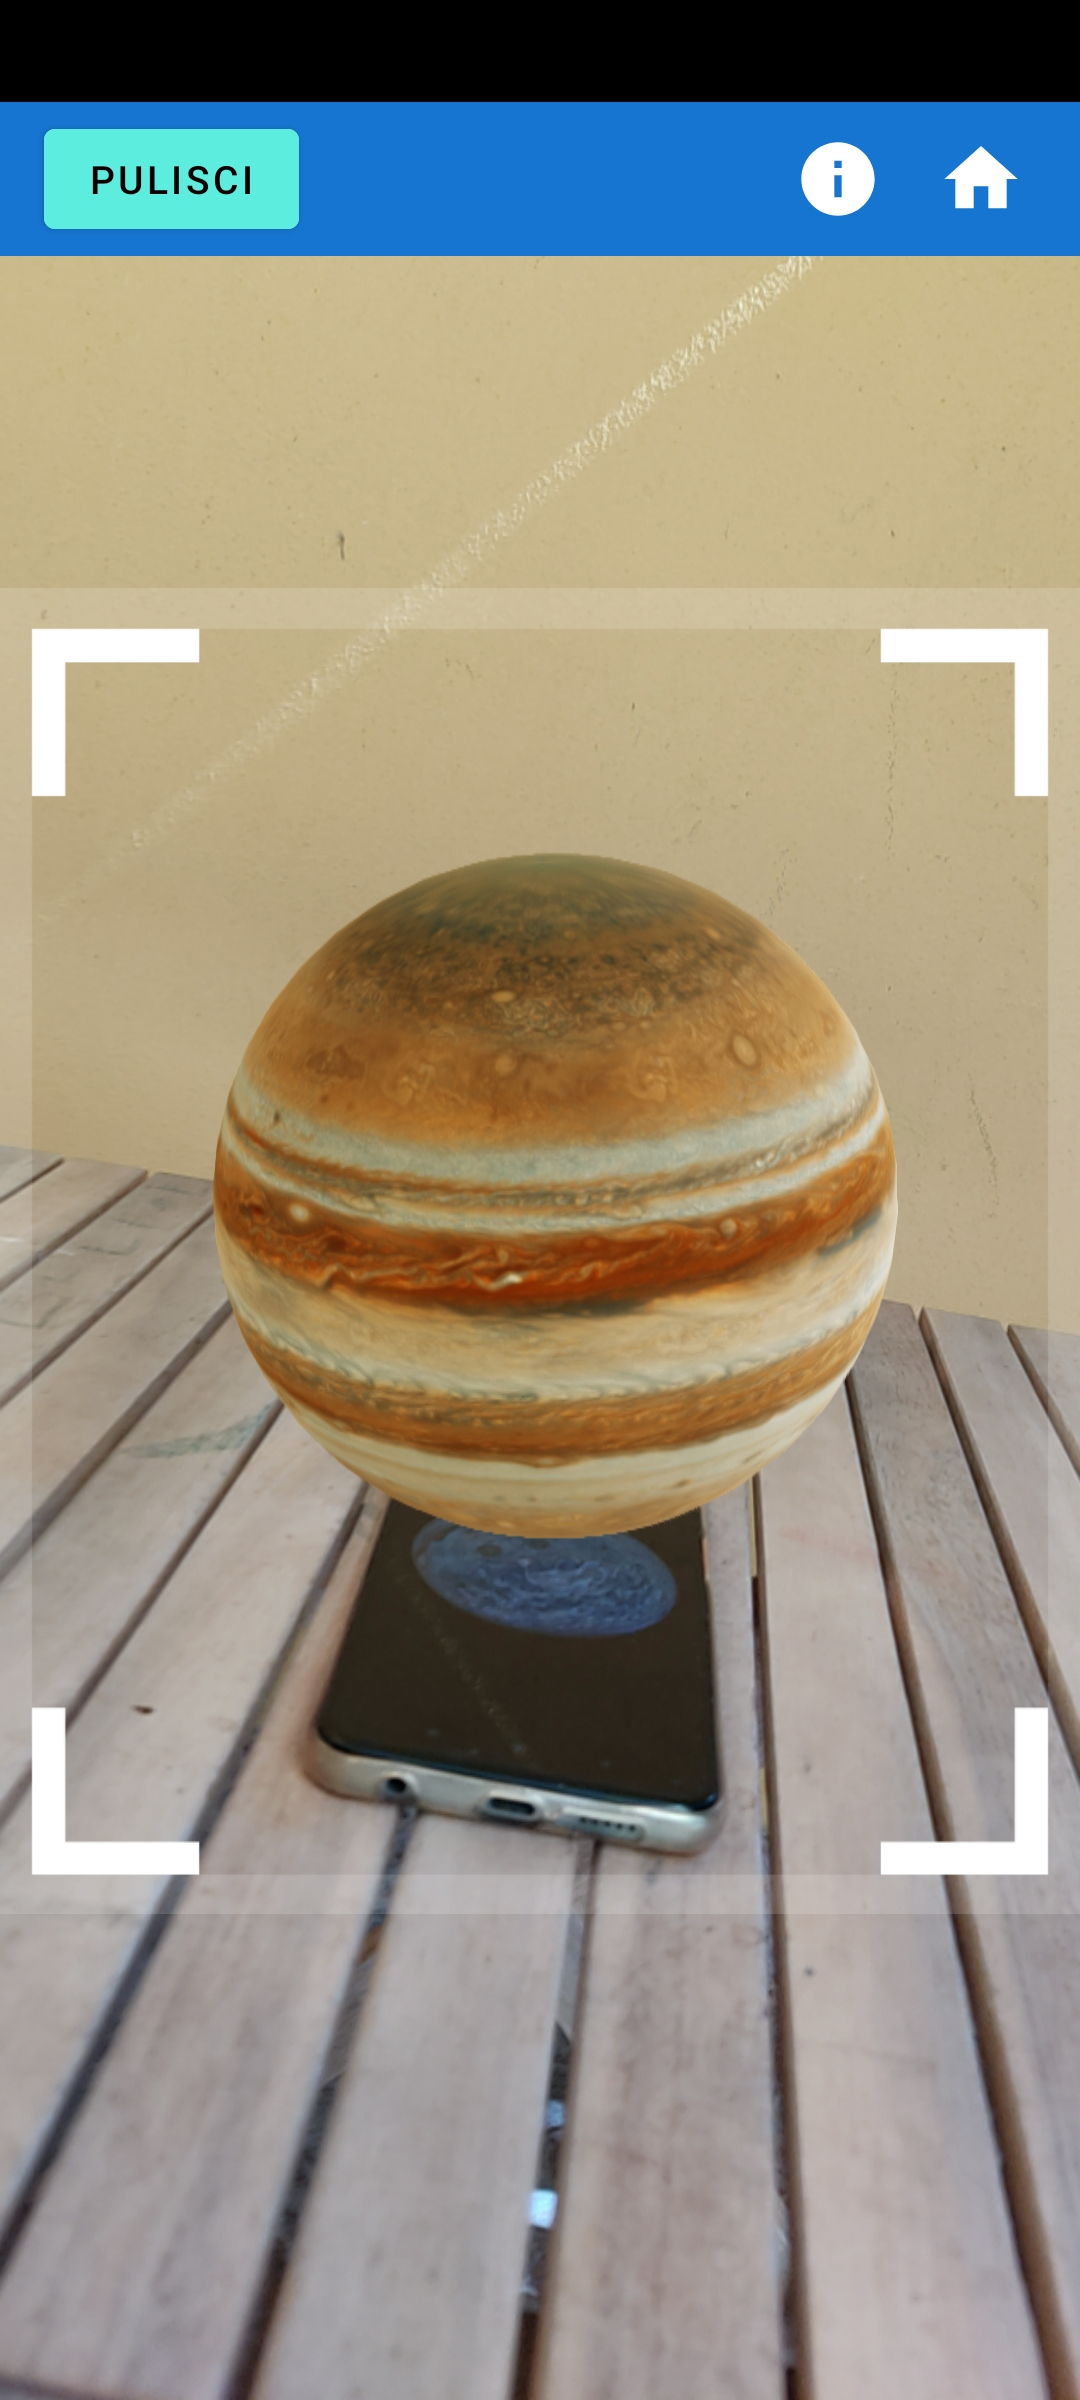
\includegraphics[width=0.28\textwidth]{../../resources/images/AnchorTrackable/GioveVicino.jpg}} \,
				\subfloat[][\emph{Giove da lontano}]
				{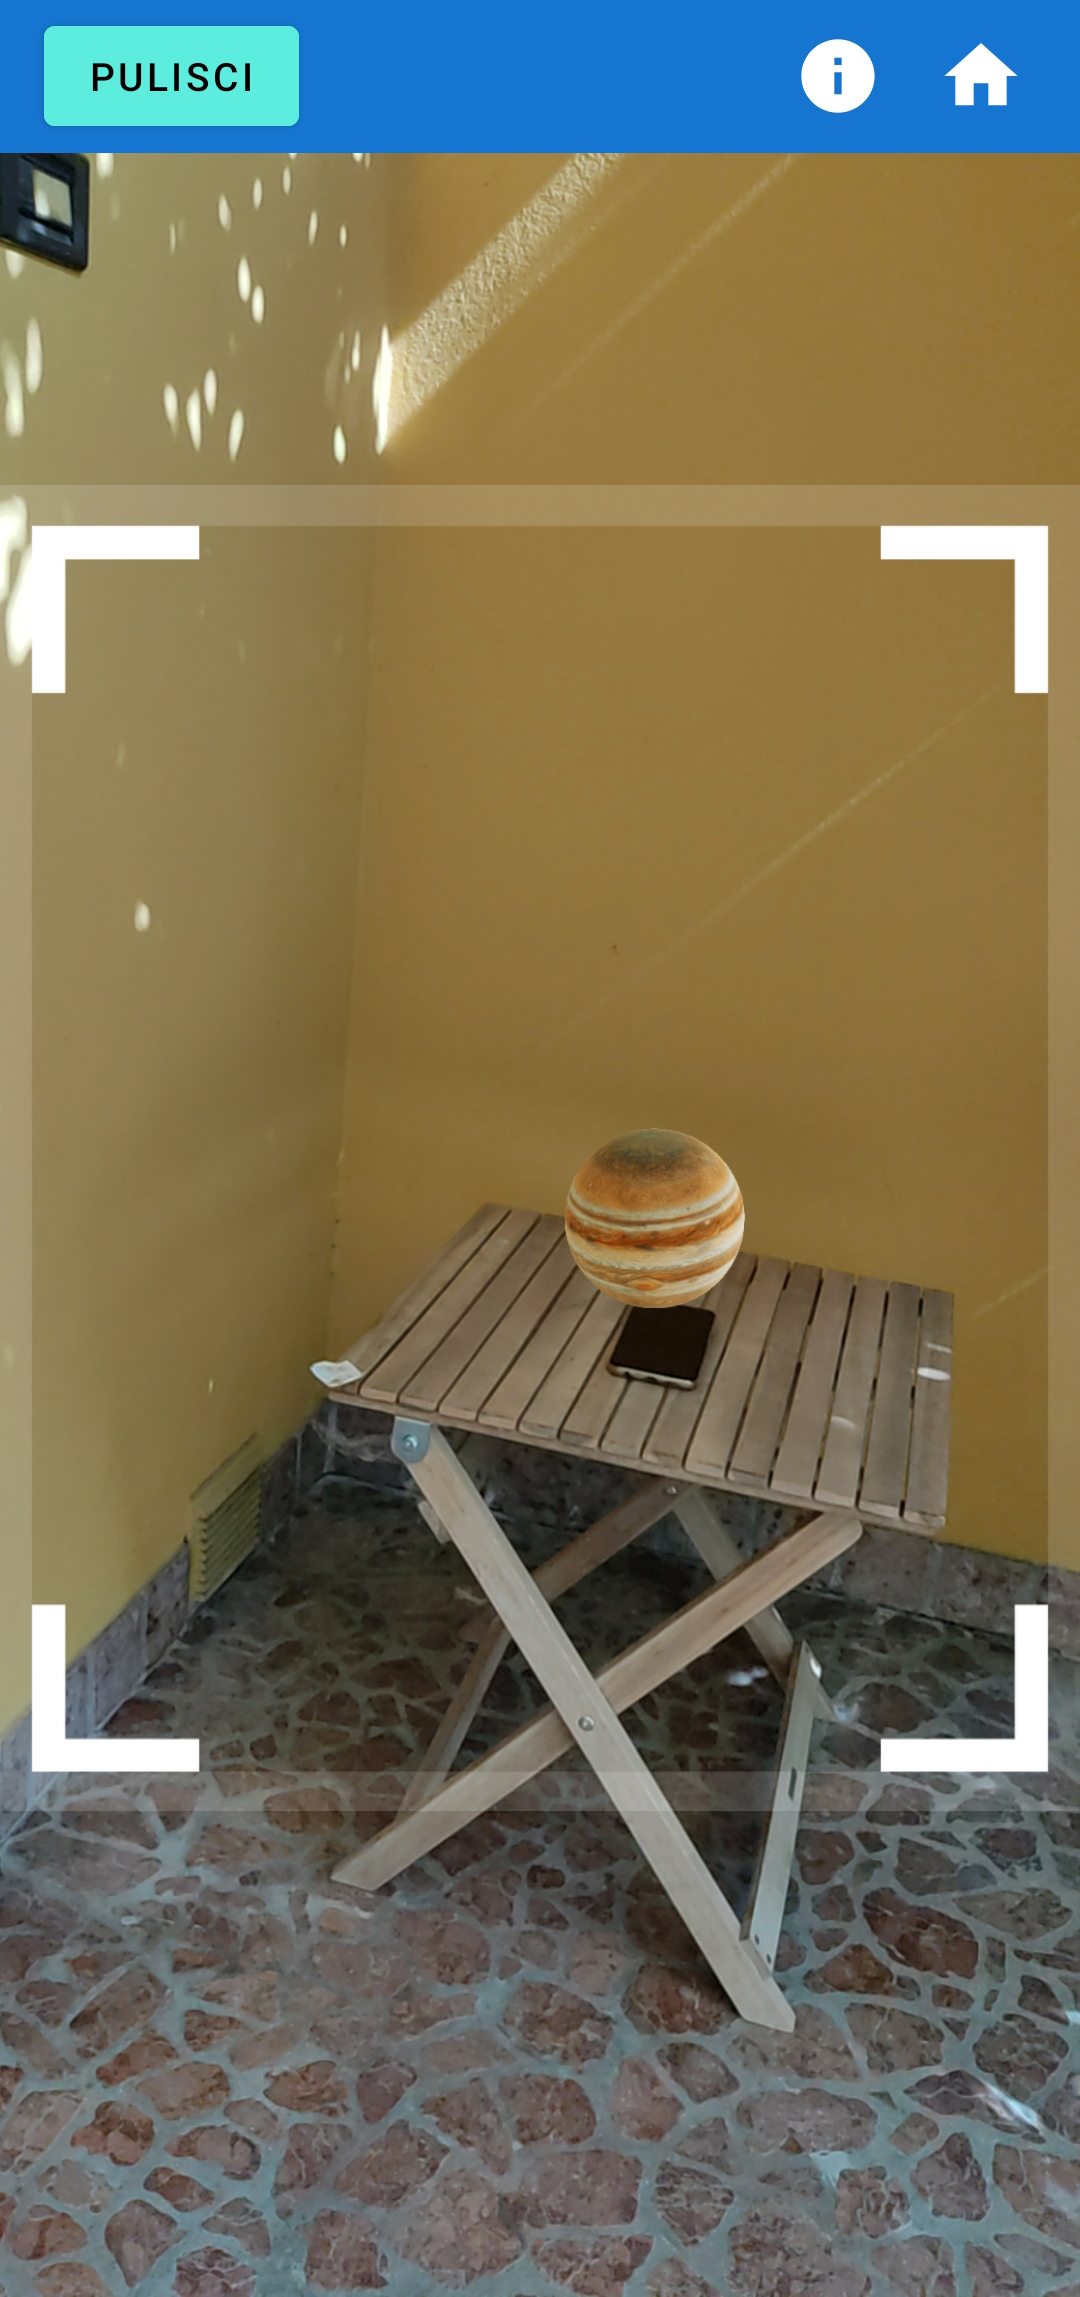
\includegraphics[width=0.28\textwidth]{../../resources/images/AnchorTrackable/GioveLontano.jpg}}
			}{Fonte: \url{https://developers.google.com/}}	
			\caption{Esempio di rilevamento in Augmented Images}
			\label{fig:augm_img}
		\end{figure}
\end{document}

	% Marco
	\documentclass[crop=false, class=book]{standalone}


\usepackage{graphicx}
\usepackage[italian]{varioref}
\usepackage{copyrightbox}



\begin{document}
	\chapter{Augmented Images}
	
	
	Le API Augmented Images in ARCore consentono di rilevare e poi manipolare le immagini presenti nel mondo reale e integrarle con elementi del mondo virtuale. \\
	\noindent
	Dopo aver fornito delle immagini, ARCore con un algoritmo che estrae dei punti caratteristici in scala di grigi dall’immagine, ripone tutti questi dettagli in uno o più database. \\
	\noindent
	Durante l’esecuzione, ARCore cerca questi punti nell’ambiente consentendo di rilevare la posizione, l’orientamento e la dimensione dell’immagine nello spazio.
	\begin{figure}
	\centering
	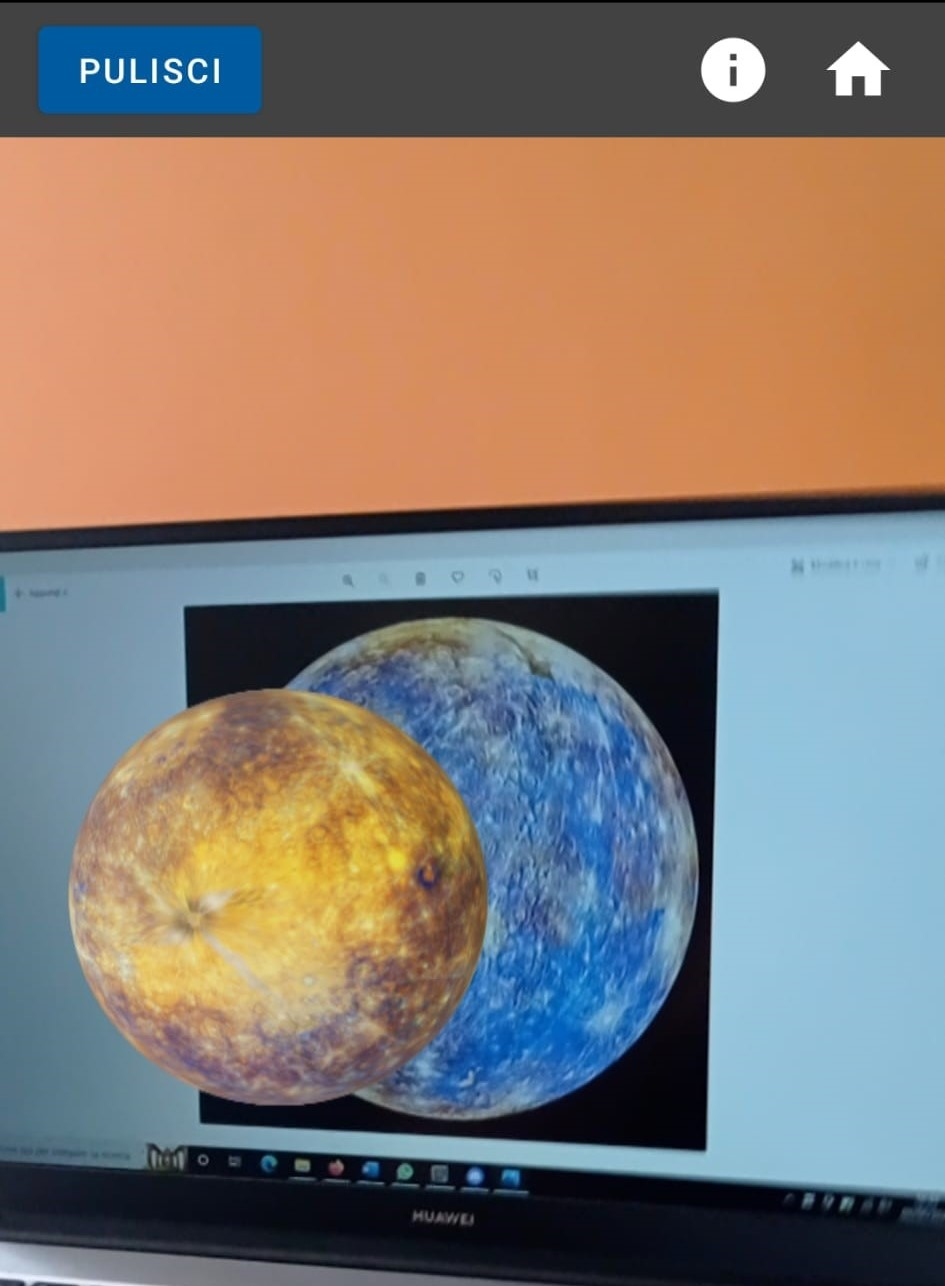
\includegraphics[width=0.5\textwidth]{./resources/images/AugmentedImages/Img1.jpeg}
	\caption{Versione in 3D di mercurio} 
	\end{figure}

	\section{Capacità}
	ARCore riesce a individuare fino a 20 immagini in contemporanea e non individua due istanze della stessa immagine. Il suo database riesce a contenere fino a 1000 immagini ed inoltre, non c’è limite al numero di database che possono essere caricati. L’unico vincolo è che si può attivare ed usare un singolo database alla volta. Quando si aggiunge un’immagine è possibile indicargli la sua grandezza nell’ambiente così da velocizzare il processo di tracciamento. \\
	\noindent
	Se non viene fornita la dimensione dell’immagine, ARCore stimerà la sua grandezza e la migliorerà durante l’esecuzione. Se viene fornita la sua dimensione ARCore ignorerà la discrepanza tra la dimensione attuale e quella segnalata e scalerà tutto secondo la dimensione dell’immagine dichiarata.\\
	\noindent
	ARCore è in grado di rilevare e tracciare sia immagini fisse, come ad esempio un poster nel muro, oppure immagini in movimento, come ad esempio un utente che ha l’immagine nella sua mano.
	Una volta che l’immagine viene rilevata ARCore continua ad ottenere informazioni ed a rifinire la sua stima dell’immagine nell’ambiente (\verb|FULL_TRACKING|).
	Se l’immagine si muove fuori dall’inquadratura ARCore continua a stimare la sua posizione assumendo che l’immagine sia statica e non si muova nell’ambiente (\verb|LAST_KNOWN_POSE|).

	\newpage
	\noindent
	L’immagine deve rispettare i seguenti requisiti:
	\begin{itemize}
		\item Essere visibile almeno al 25\% nell'inquadratura
		\item Essere piatta e non accartocciata
		\item Essere libera da ogni oggetto tra la fotocamera e l'immagine. Non deve essere oscurata, vista troppo angolata oppure vista quando la fotocamera si muove troppo velocemente
	\end{itemize}
	
	\noindent
	In base alle funzionalità di ARCore abilitate, la batteria potrebbe scaricarsi più velocemente e può aumentare l’utilizzo della CPU. E’ consigliato disabilitare le funzionalità non utilizzate per preservare la batteria e rendere più leggero il carico della CPU.
	
	\section{Creazione del database}
	Esistono due metodi per creare un database di immagini che verranno successivamente usate da ARCore.
	\\
	
	\noindent
	Il primo metodo consiste nell'importare un database creato in precedenza con il tool \textit{arcoreimg} descritto nel paragrafo~\vref{sec:arcoreimg}.
	Per importarlo si procede come descritto dal listing~\vref{lst:ai_dbimport}, tratto dalla guida ufficiale.
	
	\begin{center}
		\begin{minipage}{0.95\textwidth}
			\begin{lstlisting}[caption={Importazione database.}, label={lst:ai_dbimport}, language=Kotlin]
			val imageDatabase = this.assets.open("example.imgdb").use {
		 	
		 		AugmentedImageDatabase.deserialize(session, it)
			}
			\end{lstlisting}
		\end{minipage}
	\end{center}
	
	\noindent
	Il secondo metodo consiste nel creare un database a runtime partendo con delle immagini contenuti nella cartella \verb|assets| dell’applicazione, come descritto dal listing~\vref{lst:ai_dbruntime}.
	\\
	\begin{center}
		\begin{minipage}{0.95\textwidth}
			\begin{lstlisting}[caption={Creazione del database.}, label={lst:ai_dbruntime}, language=Kotlin]
			val imageDatabase = AugmentedImageDatabase(session)
			
			val bitmap = assets.open("dog.jpg").use { BitmapFactory.decodeStream(it) }
			
			// Se la dimensione fisica dell'immagine è sconosciuta usa il metodo 
			// addImage(String, Bitmap), che diminuisce il tempo di rilevamento dell'immagine.
			
			val imageWidthInMeters = 0.10f // 10 cm
			
			val dogIndex = imageDatabase.addImage("dog", bitmap,  imageWidthInMeters)
			\end{lstlisting}
		\end{minipage}
	\end{center}
	
	\section{Tool arcoreimg}	
	\label{sec:arcoreimg}
	Per la creazione del database a tempo di compilazione si può utilizzare il tool \textit{Arcoreimg} fornito nel SDK di Google ARCore per Android. \\
	\noindent
	Oltre a creare il database, questo strumento permette di calcolare quanto è adatta per essere individuata dalla libreria.
	Per valutarla bisogna usare il proprio terminale e scrivere:
	\begin{center}
		\begin{minipage}{0.95\textwidth}
			\begin{lstlisting}[caption={Valutazione delle immagini}, label={lst:ai_arcoreimg}, language=Kotlin, basicstyle=\ttfamily\scriptsize]
			arcoreimg.exe eval-img --input_image_path=image.png
			\end{lstlisting}
		\end{minipage}
	\end{center}
	\noindent
	Se si ottiene un punteggio superiore a 75 su 100 allora l'immagine è utilizzabile all'interno del database e sarà individuata facilmente.\\
	\noindent
	Per avere un buon punteggio bisogna che le immagini non abbiano molte ripetizioni geometriche (come i QR code). Più le immagini hanno elementi dalle forme e colori diversi, più sarà facile individuarle. Si veda la figura~\vref{fig:ai_example} per un esempio sulla qualità delle immagini.
	
	\begin{center}
		\begin{figure}[htp]
			\centering
			\copyrightbox[b]{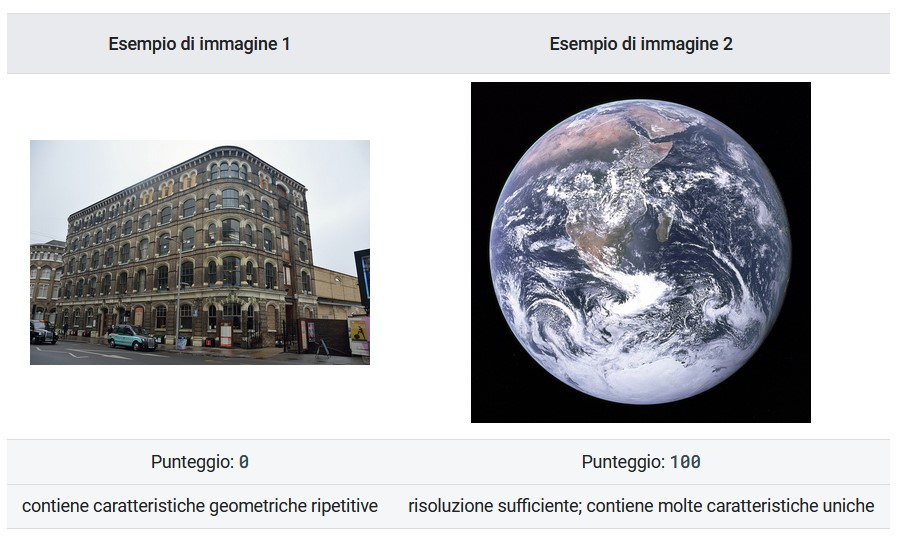
\includegraphics[width=0.9\textwidth]{./resources/images/AugmentedImages/Img2.jpg}}%
			{Fonte: \url{https://developers.google.com}}
			\caption{Esempio sulla qualità delle immagini.}
			\label{fig:ai_example}
		\end{figure}
	\end{center}
	
	\section{Abilitare il tracciamento delle immagini}
	Per abilitare il tracciamento delle immagini bisogna modificare la configurazione della sessione per impostare il database da utilizzare, come descritto dal listing~\vref{lst:ai_session}
	
	\begin{center}
		\begin{minipage}{0.95\textwidth}
			\begin{lstlisting}[caption={Creazione della sessione ARCore con Augmented Images.}, label={lst:ai_session}, language=Kotlin]
			val config = Config(session)
			
			config.augmentedImageDatabase = imageDatabase
			
			session.configure(config)
			\end{lstlisting}
		\end{minipage}
	\end{center}



\end{document}

	\documentclass[crop=false, class=book]{standalone}


\usepackage{graphicx}
\usepackage[italian]{varioref}
\usepackage{copyrightbox}


\begin{document}
	\chapter{Instant Placement}
	L'API di posizionamento istantaneo consente di posizionare gli oggetti nell’ambiente prima ancora che venga spostato il dispositivo e che vengano individuati i piani. \\
	\noindent
	Dopo che l’utente ha posizionato l’oggetto, la sua posizione viene perfezionata in tempo reale mentre l’utente si muove nell’ambiente.
	\\
	\noindent
	Successivamente, quando ARCore è in grado di identificare con precisione l’ubicazione dell’oggetto nello spazio, viene cambiata la sua posizione e dimensione per rispettare la scala dell’ambiente.
	\begin{figure}
		\centering
		\copyrightbox[b]{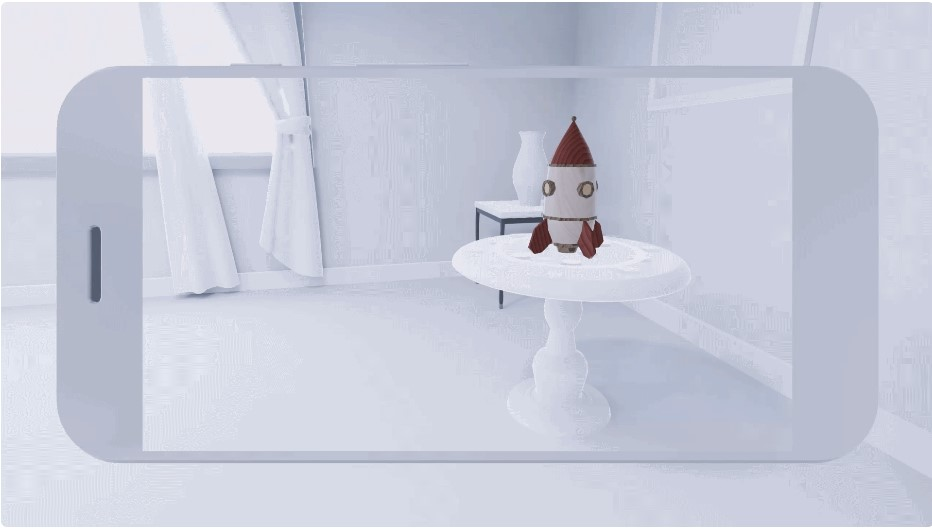
\includegraphics[width=0.6\textwidth]{./resources/images/InstantPlacement/InstantPlacementImg.jpg} }%
		{Fonte: \url{https://developers.google.com}}
		\caption{dfgdf}
		\label{fig:light_effects}
	\end{figure}
	\\
	\noindent
	Per abilitare l’instant placement bisogna creare una sessione configurata per supportare l’instant placement, come descritto dal listing~\vref{lst:ip_session}
		
	\begin{center}
		\begin{minipage}{0.95\textwidth}
			\begin{lstlisting}[caption={Descrizione del listing.}, label={lst:ip_session}, language=Kotlin]
			fun createSession() {
				
			val session = Session(applicationContext);
			
			val config = Config(session)
			
			config.instantPlacementMode = Config.InstantPlacementMode.LOCAL_Y_UP
			
			session.configure(config)
		}
		\end{lstlisting}
		\end{minipage}
	\end{center}

\end{document}
	\documentclass[crop=false, class=book]{standalone}


\usepackage{graphicx}
\usepackage[italian]{varioref}
\usepackage{copyrightbox}


\begin{document}
	\chapter{Recording e Playback}
	
	Solitamente quando si utilizza un’applicazione AR ci si trova ad essere in prima persona nell’ambiente il cui deve essere utilizzata.	L'API \textit{Recording and Playback} consente di utilizzare i servizi di ARCore anche su un feed video non in tempo reale. Più precisamente si può fornire un video e ARCore lo tratterà come se fosse un video registrato in tempo reale \cite{google2022rec}.
	\\
	\noindent
	L'API Recording archivia il video stream, i dati IMU o qualsiasi altri metadati personalizzati che scegli di salvare in un file MP4. Successivamente l’utente potrà sceglie se usare un video dal vivo oppure un video preregistrato.
 
	\section{Compatibilità}
	ARCore è necessario per utilizzare API Recording and Playback perché serve per registrare i dati nel file MP4. I file MP4 registrati, utilizzando questa funzionalità, sono essenzialmente file video con dati aggiuntivi e possono essere visualizzati utilizzando qualsiasi video player. Per ispezionare i file è possibile usare, per esempio, il player Exoplayer di Android.
	 
	\section{Salvataggio di dati video e AR}
	ARCore salva le registrazioni in formato MP4. All’interno di questo file sono contenuti più tracciati video registrati con la codifica H.264 e dati vari. La prima traccia video viene solitamente registrata ad una risoluzione di 640x480 (VGA) e questa traccia verrà usata per il motion tracking come fonte di video primaria.
	\\
	\noindent
	Nel caso si voglia una risoluzione migliore, bisogna configurare una nuova fotocamera che abbia la risoluzione desiderata.
	In questo caso ARCore richiederà un feed in qualità 640x480 e un feed in alta risoluzione. Questo potrebbe rallentare la propria applicazione a causa di un maggiore utilizzo della CPU. Verrà inoltre selezionata la risoluzione personalizzata come fonte primaria del video che verrà salvato nel file MP4.
	\\
	\noindent
	La seconda traccia del file MP4 è una visualizzazione della mappa della profondità della fotocamera. Si tratta di un video ricavato dal sensore di profondità del proprio dispositivo e successivamente convertito in valori dei canali RGB.
	\\
	\noindent
	ARCore registra anche le misurazioni del giroscopio e dell’accelerometro del dispositivo. Inoltre, vengono salvati anche altri dati, tra cui alcuni considerati sensibili. Questi dati sono la versione SDK di Android, il fingerprint del dispositivo, informazioni addizionali sui sensori usati e, se il ARCore Geospatial API è attivo, la posizione stimata, i dati del magnetometro e della bussola.
	 
	\section{Recording}
	Per iniziare una sessione di registrazione inizialmente viene creata la sessione di ARCore, viene specificato il file di output e alcune configurazioni sulla registrazione. Infine inizia la registrazione. Per concludere la registrazione è necessario invocare il metodo \verb|stopRecording()| sull'istanza \verb|session|. Si veda il listing~\vref{lst:pr_session} tratto dalla documentazione ufficiale Google \cite{google2022rec2}.
	
	\begin{center}
		\begin{minipage}{0.95\textwidth}
			\begin{lstlisting}[caption={Creazione della sessione per recording.}, label={lst:pr_session}, language=Kotlin]
val session = Session(context)
			// Creazione della sessione ARCore.
			val destination = Uri.fromFile(File(context.getFilesDir(),"recording.mp4"))
			
			val recordingConfig = RecordingConfig(session)
							.setMp4DatasetUri(destination)
							.setAutoStopOnPause(true)
							
			session.startRecording(recordingConfig)
			
			// Chiamata al metodo resume() per iniziare la registrazione.
			session.resume()
			
			// Ferma il recording.
			session.stopRecording()
			\end{lstlisting}
		\end{minipage}
	\end{center}	

	\noindent
	Tramite il metodo \verb|getRecordingStatus()| della classe \verb|Session| è possibile verificare lo stato della registrazione, tramite il valore di tipo \verb|RecordingStatus| restituito.


	\section{Playback}
	Il playback di una sessione precedentemente registrata è possibile tramite il metodo \verb|setPlaybackDatasetUri()| della classe \verb|Session|. La riproduzione inizia con la chiamata al metodo \verb|session.resume()| e può essere messa in pausa tramite il metodo \verb|session.pause()|. Il listing~\vref{lst:playback} mostra la riproduzione di una sessione.
	\begin{center}
		\begin{minipage}{0.95\textwidth}
			\begin{lstlisting}[caption={Creazione della sessione per il playback.}, label={lst:playback}, language=Kotlin]
			// Configura la sessione ARCore.
			val session = Session(context)
			
			// Specifica l'Uri del file da riprodurre.
			val recordingUri = Uri.fromFile(File(context.filesDir, "recording.mp4"))
			session.playbackDatasetUri = recordingUri
			...
			
			// Inizia la riproduzione dall'inizio.
			session.resume()
			...
			
			// Metti in pausa la riproduzione del file.
			session.pause()
			...
			
			\end{lstlisting}
		\end{minipage}
	\end{center}	
	\noindent
	Tramite il metodo \verb|setPlaybackDatasetUri(Uri mp4DatasetUri)| della classe \verb|Session| è possibile riprodurre dall'inizio il file già riprodotto, specificando lo stesso Uri, oppure iniziare il playback di un nuovo file MP4, come descritto dal listing~\vref{lst:playback2}.
	\begin{center}
		\begin{minipage}{0.95\textwidth}
			\begin{lstlisting}[caption={Esempi di utilizzo del playback.}, label={lst:playback2}, language=Kotlin]
			// Riproduzione dall'inizio del file
			session.pause()
			// Specificando lo stesso Uri la riproduzione inizia da capo.
			session.playbackDatasetUri = previousRecordingUri
			// Il file viene riprodotto dall'inizio
			session.resume() 
			
			// Riproduzione di un nuvo file
			session.pause()   
			// Specifica un nuovo dataset da utilizzare.
			session.playbackDatasetUri = newRecordingUri
			// Inizia il playback del nuovo file.
			session.resume()  
				
			\end{lstlisting}
		\end{minipage}
	\end{center}	
	\noindent
	Tramite il metodo \verb|getPlaybackStatus()| della classe \verb|Session| è possibile verificare lo stato della registrazione, tramite il valore di tipo \verb|PlaybackStatus| restituito.
	
	\section{Dati aggiuntivi}
	Durante la registrazione di una sessione ARCore è possibile aggiungere dati aggiuntivi oltre ai dati video e dei sensori, da ricavare poi durante il playback della registrazione. Tale funzionalità può essere utile ad esempio per registrare una stanza e gli oggetti presenti in essa, e aggiungere durante il playback altri oggetti, come una lampada, senza essere presenti fisicamente nella stanza.
	 
	\newpage
	\noindent
	I dati aggiuntivi devono essere inseriti in un oggetto di tipo \verb|Track| identificato da un \verb|UUID|, che rappresenta un identificativo unico e immutabile. La traccia \verb|Track| deve poi essere inserita nella configurazione della sessione ARCore per la registrazione, come descritto dal listing~\vref{lst:UUID} tratto dalla documentazione ufficiale. Inoltre, è possibile aggiungere alla traccia dei dati di identificazione aggiuntivi, come una descrizione sul luogo e l'orario in cui la registrazione è stata fatta. Se la registrazione deve essere compatibile con altre applicazioni, essa può inoltre essere associata con un identificativo \verb|MIME| che descrive il tipo di dati registrati sulla traccia.
	\begin{center}
		\begin{minipage}{0.95\textwidth}
			\begin{lstlisting}[caption={Aggiunta di una traccia alla sessione ARCore.}, label={lst:UUID}, language=Kotlin]
			// Inizializza una nuova traccia con un identificativo UUID.
			// Tale identificativo sarà necessario per recuperare i dati aggiuntivi durante il playback.
			val trackUUID = UUID.fromString("de5ec7a4-09ec-4c48-b2c3-a98b66e71893")
			val track = Track(session).setId(trackUUID)
			
			// Viene aggiunta come descrizione il luogo in cui è stata effettuata.
			val customTrackData: ByteArray = "airport".toByteArray()
			track.setMetadata(ByteBuffer.wrap(customTrackData))
			
			// Imposta un tipo MIME per essere compatibile con altre applicazioni.
			track.setMimeType("text/csv")
			
			// Aggiunge l'oggetto Track alla configurazione della sessione.
			recordingConfig.addTrack(track)  
			
			\end{lstlisting}
		\end{minipage}
	\end{center}

	\noindent
	Durante il playback, è possibile recuperare le tracce aggiuntive tramite il metodo \verb|getUpdatedTrackData()| che restituisce una \verb|Collection| di oggetti \verb|TrackData|, dai quali è possibile estrarre i dai aggiuntivi inseriti durante il recording. Si veda il listing~\vref{lst:playback_retrieve} per un esempio di utilizzo.
	\begin{center}
		\begin{minipage}{0.95\textwidth}
			\begin{lstlisting}[caption={Recupero della traccia aggiuntiva durante il playback.}, label={lst:playback_retrieve}, language=Kotlin]
			// Recupero della collection di tracce aggiuntive.
			val trackDataList:Collection<TrackData> = frame.getUpdatedTrackData(trackUUID)
			
			// Ispezione delle tracce restituite dal metodo.
			for (trackData in trackDataList) {
				// Dati della traccia
				val bytes = trackData.data
			}
				
			\end{lstlisting}
		\end{minipage}
	\end{center}





\end{document}


	
	% Mattia
	\documentclass[crop=false, class=book]{standalone}

%impostazioni lingua
\usepackage[T1]{fontenc}
\usepackage[utf8]{inputenc}
\usepackage[english,italian]{babel}

%sistema i margini
\usepackage{geometry}
\geometry{a4paper,top=2.2cm,bottom=2.2cm,left=3cm,right=3cm, heightrounded}

%interlinea 1.5
\usepackage{setspace}
\onehalfspacing

%gestione delle testatine
\usepackage{fancyhdr}
\pagestyle{fancy}
\lhead{}
\chead{}
\rhead{Titolo}
\lfoot{}
\cfoot{\thepage}
\rfoot{}
\renewcommand{\headrulewidth}{0.4pt}

%formattazione titoli paragrafo
\usepackage{titlesec}
\titleformat{\chapter}[block]{\normalfont\huge\bfseries}{\thechapter.}{0.7em}{\huge}

%pacchetti per i riferimenti in bibliografia
\usepackage[autostyle,italian=guillemets]{csquotes}
\usepackage[style=numeric,citestyle=numeric-comp,backend=biber]{biblatex}

%risorsa che contiene la bibliografia
\addbibresource{./bibliografia.bib}

%pacchetto per immagini
\usepackage{graphicx}
\usepackage{subfig}

\usepackage[italian]{varioref}
\usepackage{copyrightbox}
\usepackage{url}


\usepackage{lipsum}

\begin{document}
	\chapter{Augmented faces}
	L'API \textit{Augmented Faces} permette di identificare i volti umani e le varie parti che lo compongono tramite Intelligenza Artificiale, per sovrapporre ad essi modelli 3D come maschere, occhiali, cappelli utilizzando solo la fotocamera frontale \cite{google2022faces}. 
	Questa libreria permette ottenere un \textit{face mesh}, una rappresentazione virtuale composta da una maglia di punti che riproduce il profilo del volto \cite{oufqir2020arkit}. Oltre ad essa, l'API fornisce un \textit{center pose} e tre \textit{region pose}, come descritti dalla figura~\vref{fig:augm_faces} tratte dalla documentazione ufficiale.
	\paragraph*{Face mesh}
		Consiste in una rete di 468 punti, che permette di posizionare una texture sul volto. Essa viene tracciata come un piano, per permettere all'immagine virtuale di seguire il volto anche se in movimento, come spiegato in \cite{googleblog2019faces}.
	\paragraph*{Center pose}
		Rappresenta il centro del volto, posizionato dietro il naso. Utile per il rendering di oggetti virtuali da posizionare sopra la testa.
	\paragraph*{Region pose}
		Identifica una regione rilevante del volto, come i lati destro o sinistro della fronte, oppure il naso. Sono utili per il rendering di oggetti virtuali da posizionare sul naso o attorno agli orecchi.
	
	\begin{figure}
		\centering
			\subfloat[][\emph{Esempio di face mesh}]
			{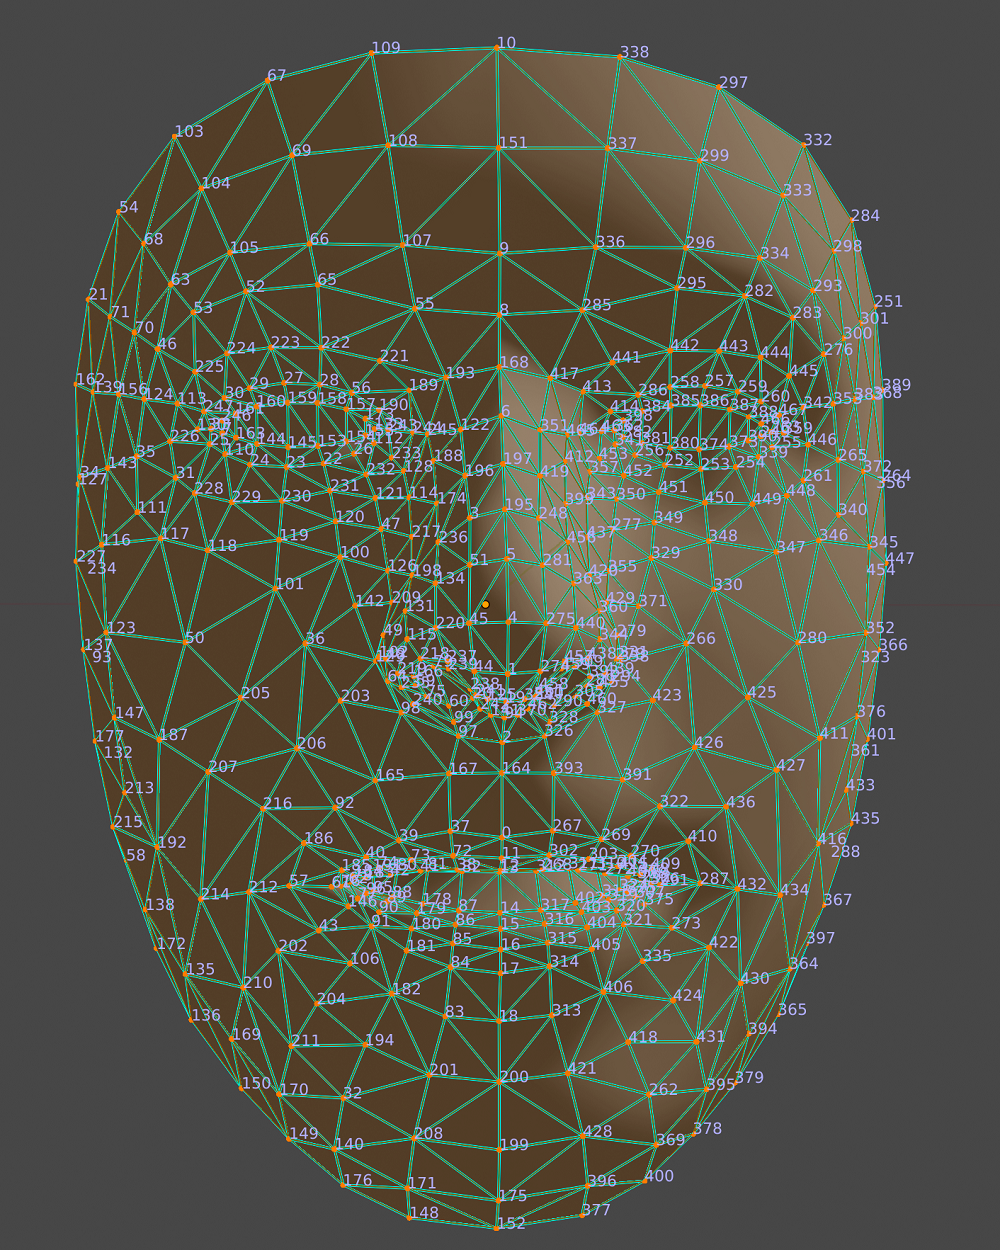
\includegraphics[width=0.31\textwidth]{./resources/images/augmented_faces/face_mesh}}  \quad
			\subfloat[][\emph{Posizione del center pose}]
			{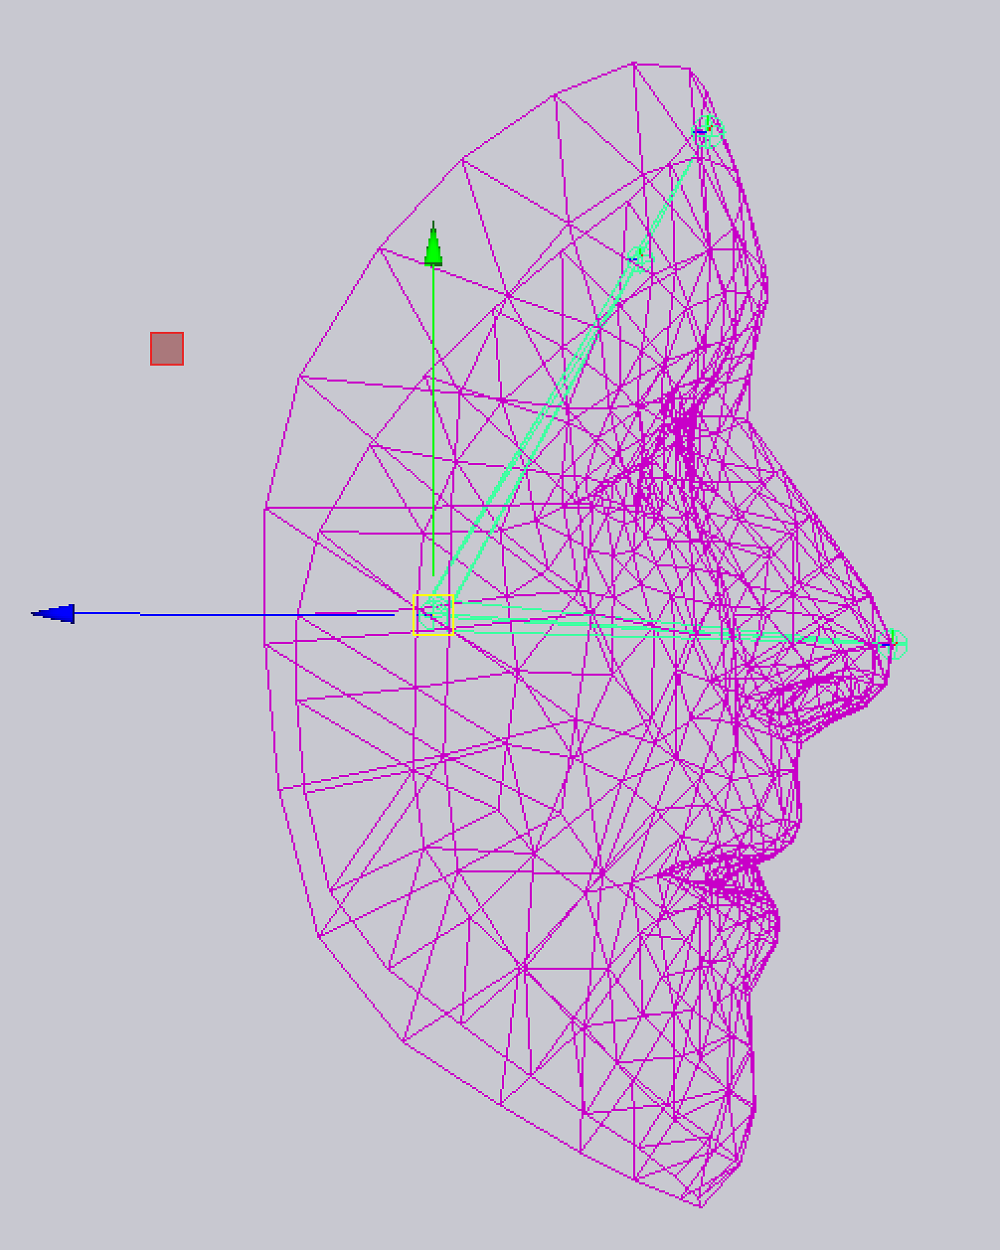
\includegraphics[width=0.31\textwidth]{./resources/images/augmented_faces/center_pose}} \quad
			\subfloat[][\emph{Posizioni di tre region pose}]
			{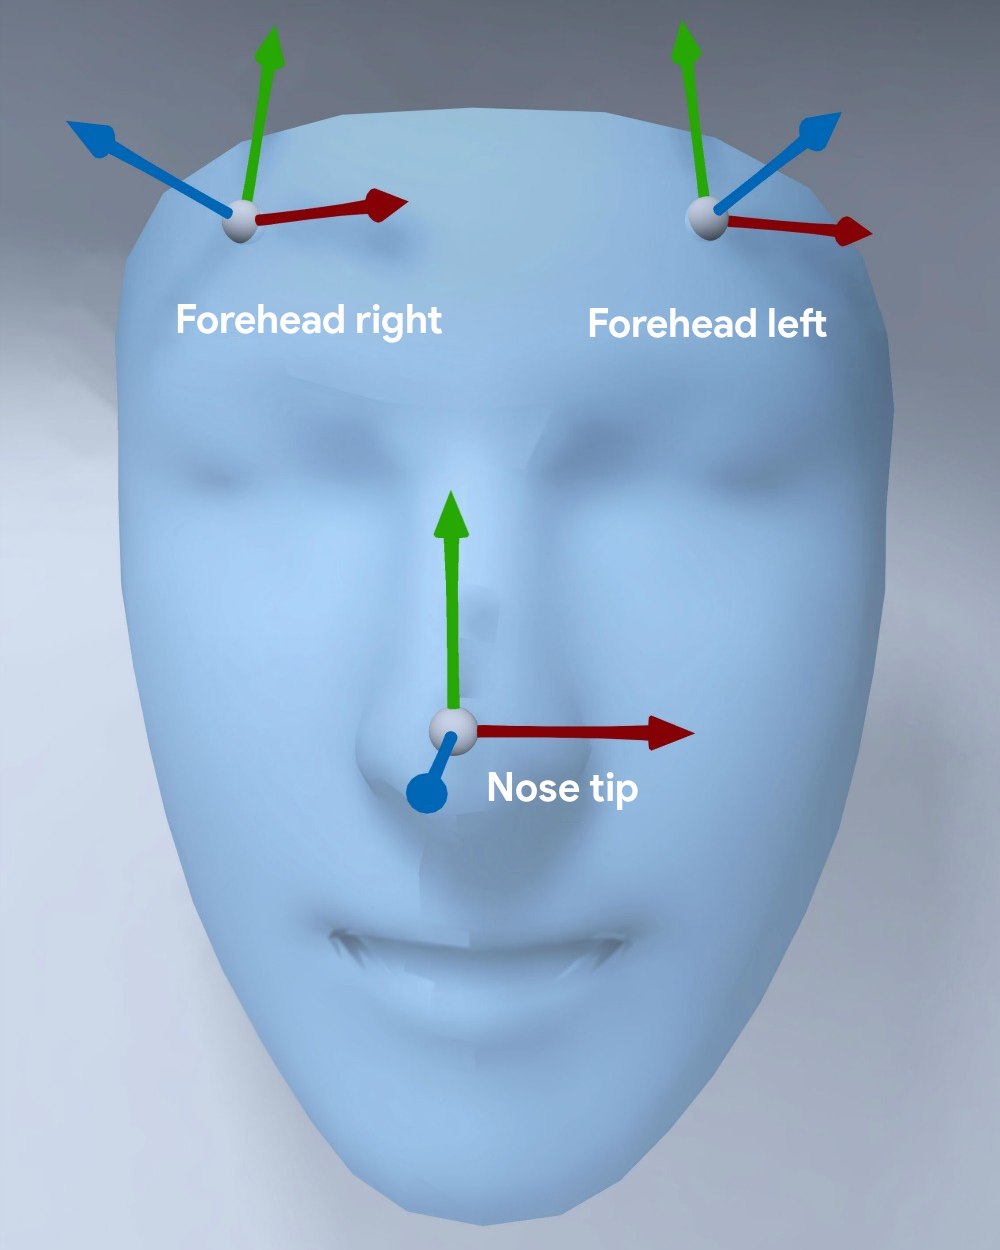
\includegraphics[width=0.31\textwidth]{./resources/images/augmented_faces/region_poses}}
		\caption{Elementi ottenuti tramite l'API Augmented Faces}
		\label{fig:augm_faces}
	\end{figure}
	
	\section{Configurazione e utilizzo}
	La configurazione della sessione ARCore deve essere effettuata selezionando la fotocamera frontale ed abilitando la modalità Augmented Face, come mostrato nel listing~\vref{lst:af_session} tratto dalla guida ufficiale Google.

	\begin{center}
		\begin{minipage}{0.95\textwidth}
			\begin{lstlisting}[caption={Configurazione della modalità Augmented Face.}, label={lst:af_session}, language=Kotlin]
			// Configura la sessione utilizzando la camera frontale.
			val filter = CameraConfigFilter(session).setFacingDirection(CameraConfig.FacingDirection.FRONT)
			val cameraConfig = session.getSupportedCameraConfigs(filter)[0]
			session.cameraConfig = cameraConfig
			
			// Abilita la modalità Augmented Face.
			val config = Config(session)
			config.augmentedFaceMode = Config.AugmentedFaceMode.MESH3D
			session.configure(config)
			\end{lstlisting}
		\end{minipage}
	\end{center}
	Da ogni frame è possibile ricavare un oggetto \verb|Trackable|, che può essere tracciato e a cui possono essere collegate degli \verb|Anchor|. Verificando lo stato di ogni oggetto \verb|Trackable| restituito, è possibile ricavare i region pose, il center pose e i vertici del face mesh, per poi procedere con il rendering degli oggetti virtuali. Si veda il listing~\vref{lst:faces_use} tratto dalla documentazione ufficiale per un possibile utilizzo.
	
	\begin{center}
		\begin{minipage}{0.95\textwidth}
			\begin{lstlisting}[caption={Utilizzo della modalità Augmented Faces.}, label={lst:faces_use}, language=Kotlin]
			// Ricava gli oggetti trackable dalla sessione ARCore
			val faces = session.getAllTrackables(AugmentedFace::class.java)
			
			// Verifica lo stato di ogni oggetto contenuto nella lista di Trackable
			faces.forEach { face ->
				if (face.trackingState == TrackingState.TRACKING) {
					// Ricava il center pose
					val facePose = face.centerPose
					
					// Ricava i region pose
					val forheadLeft = face.regionPose(AugmentedFace.RegionType.FOREHEAD_LEFT)
					val forheadRight=face.regionPose(AugmentedFace.RegionType.FOREHEAD_RIGHT)
					val noseTip = face.regionPose(AugmentedFace.RegionType.NOSE_TIP)
					
					// Ricava i vertici del face mesh
					val faceVertices = face.meshVertices
					
					// Rendering dell'oggetto virtuale
				}
			}
			\end{lstlisting}
		\end{minipage}
	\end{center}
	


	
	
\end{document}
	\documentclass[crop=false, class=book]{standalone}

%pacchetto per immagini
\usepackage{graphicx}
\usepackage{subfig}

\usepackage[italian]{varioref}
\usepackage{copyrightbox}
\usepackage{url}

\usepackage{enumitem}
\newcommand\litem[1]{\item{\bfseries #1:}}


\begin{document}
	\chapter{Cloud anchors}
	L'API ARCore \textit{Cloud Anchor} introduce i cloud anchor, un tipo speciale di anchor che permettono di condividere con altri utenti l'esperienza AR. In particolare, un dispositivo può posizionare oggetti virtuali nello spazio, e altri utenti possono vedere l'oggetto virtuale ed interagire con esso trovandosi nella stessa posizione, come spiegato da \cite{kert2021mobile}.
	\\
	Questo tipo di anchor, come spiegato dalla documentazione ufficiale \cite{google2022cloud}, trova applicazione ad esempio per creare oggetti virtuali che persistano nel mondo reale, cioè che mantengano nel tempo la posizione in cui sono stati creati, oppure per creare giochi virtuali multigiocatore in cui è importante la collaborazione tra utenti in tempo reale.
	
	\section{Funzionamento}
	La creazione e la diffusione dell'anchor avviene tramite connessione internet in quattro passaggi, descritti ad alto livello come segue. La figura~\vref{fig:cloud} tratta dalla guida ufficiale Google descrive visivamente le quattro fasi del funzionamento dei cloud anchor.
	\begin{enumerate}
		\litem{Creation} l'utente crea un anchor localmente;
		\litem{Hosting} ARCore carica i dati della mappa 3D dello spazio circostante all'anchor locale nell'ARCore Cloud Anchor, che a sua volta restituisce al dispositivo un Cloud Anchor ID univoco;
		\litem{Distribution} l'app distribuisce l'ID univoco agli altri utenti;
		\litem{Resolving} gli utenti possono utilizzare l'ID ricevuto per ricreare l'anchor quando si trovano nello stesso ambiente. L'API compara la scena del dispositivo con la mappa 3D caricata precedentemente per determinare la posizione dell'utente e visualizzare correttamente l'oggetto virtuale.
	\end{enumerate}
	
	\begin{figure}[t]
		\centering
		\subfloat[][\emph{Creazione dell'anchor locale.}]
		{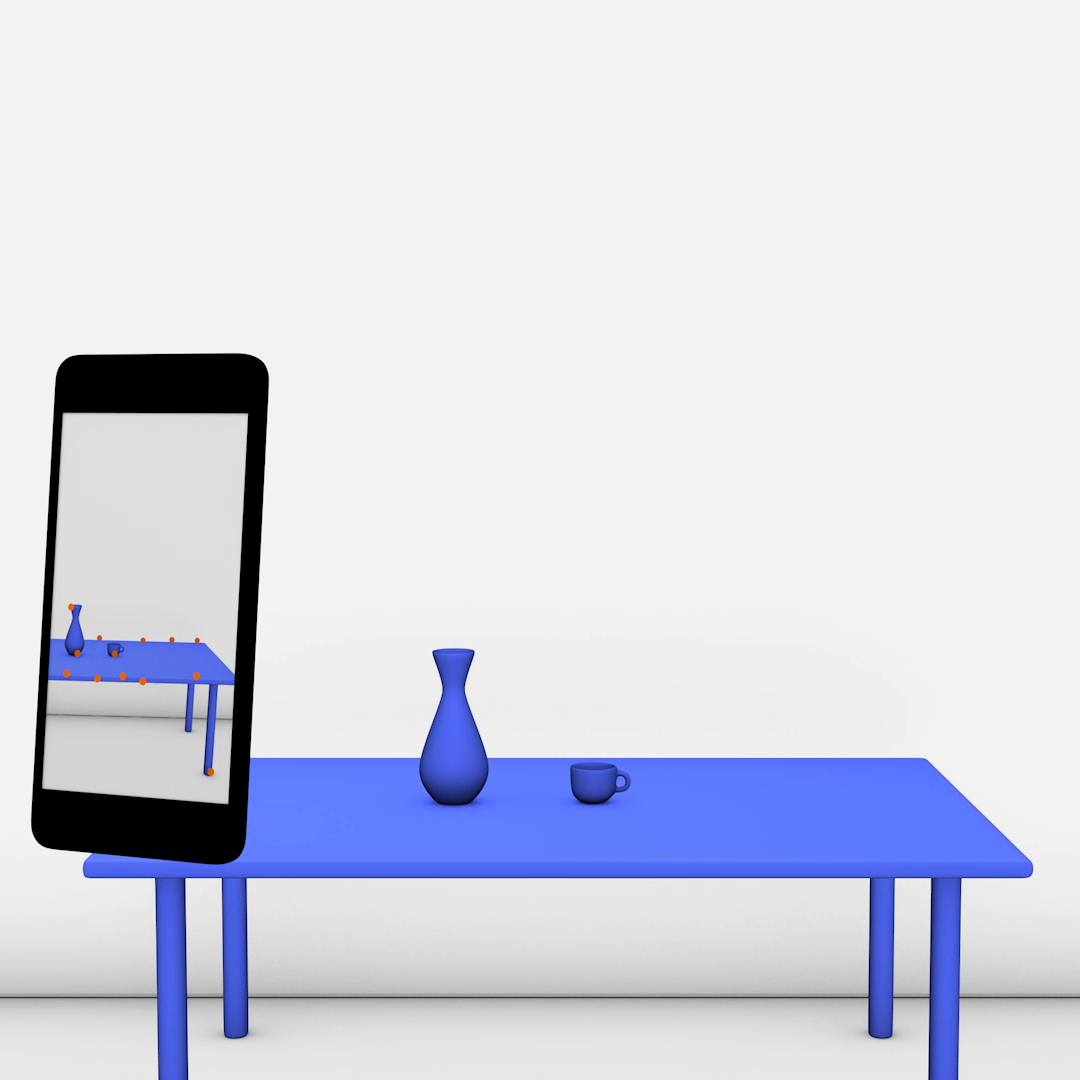
\includegraphics[width=0.45\textwidth]{./resources/images/cloud_anchors/creation}}  \quad
		\subfloat[][\emph{Hosting dell'anchor.}]
		{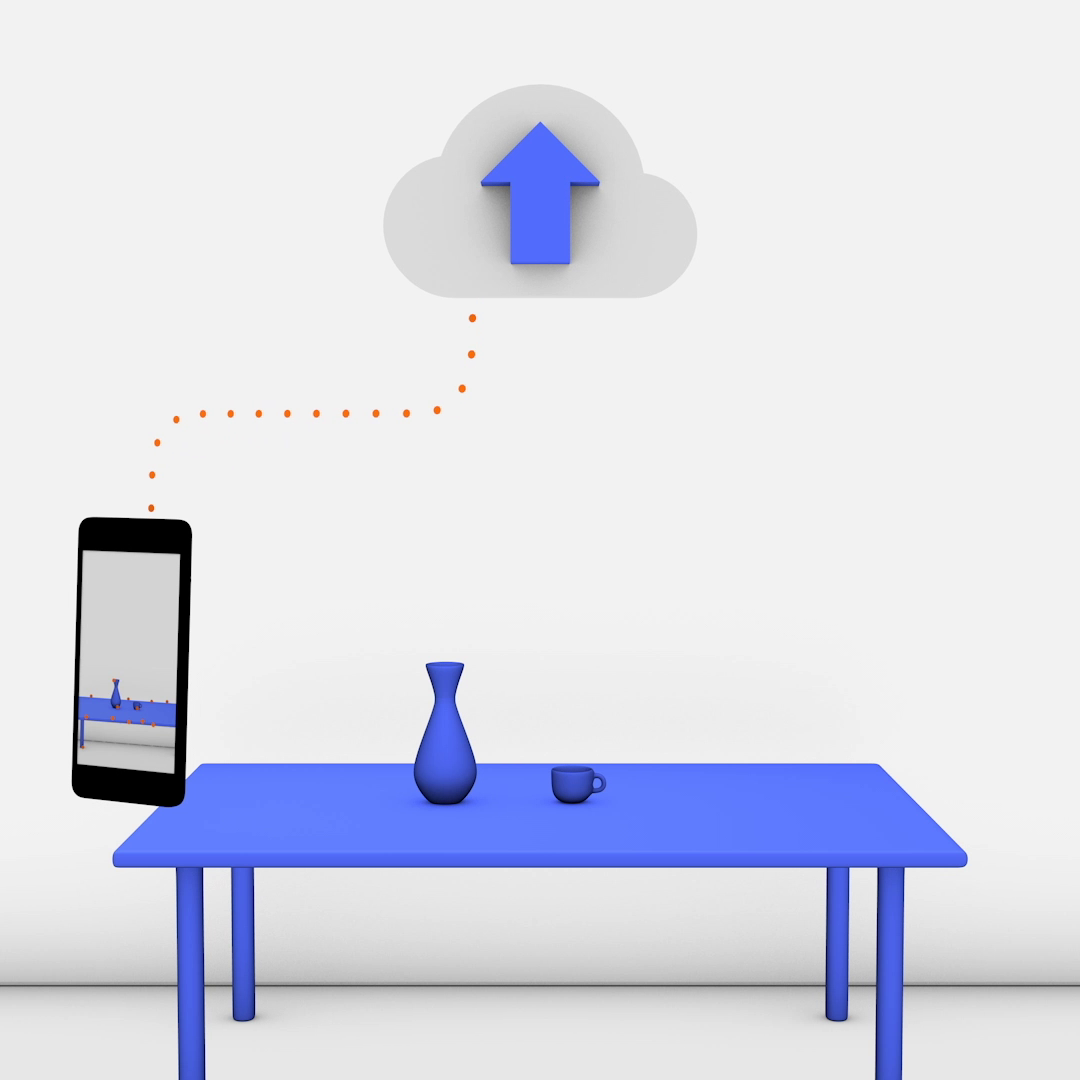
\includegraphics[width=0.45\textwidth]{./resources/images/cloud_anchors/hosting}} \\
		\subfloat[][\emph{Richiesta resolve al cloud anchor.}]
		{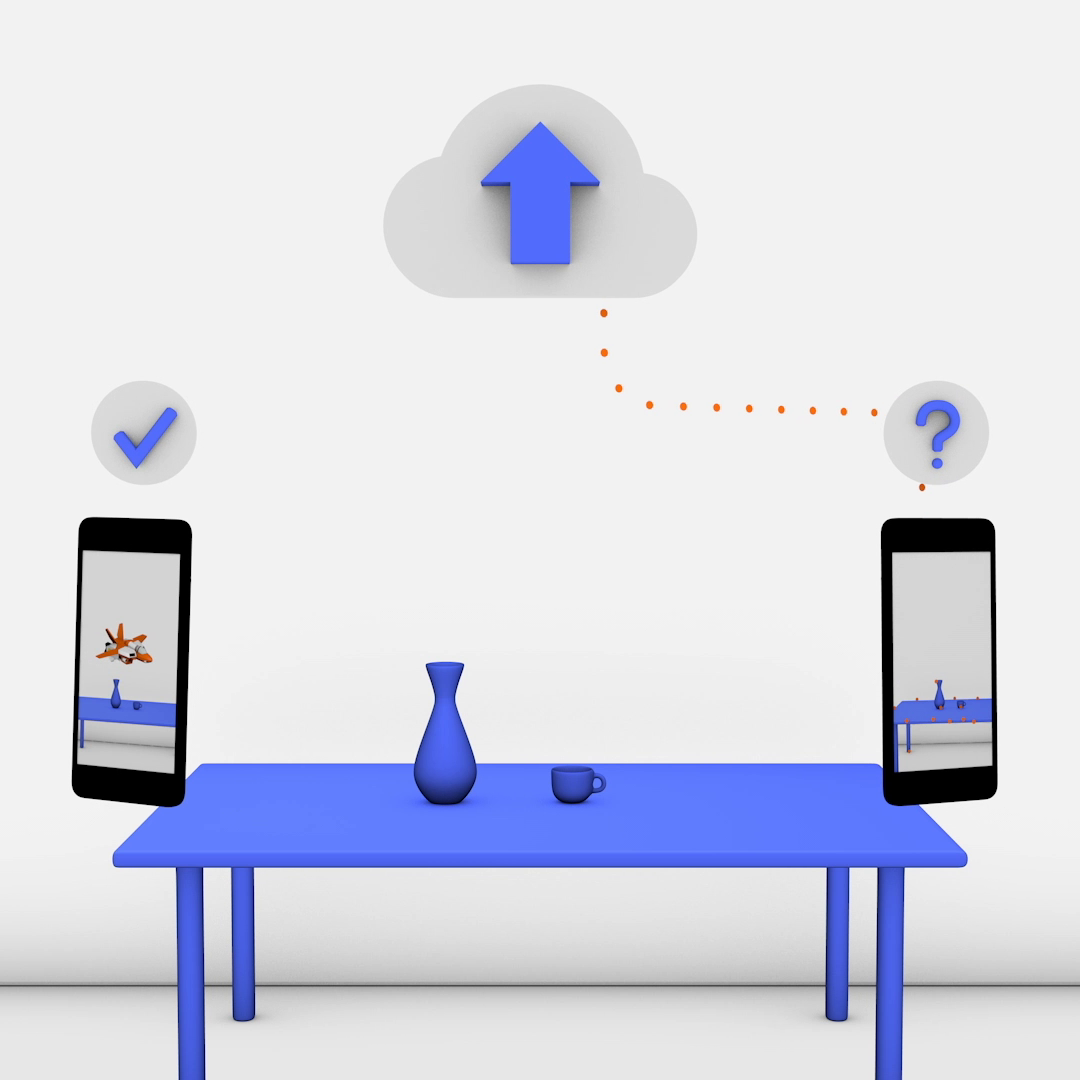
\includegraphics[width=0.45\textwidth]{./resources/images/cloud_anchors/distribution}} \quad
		\subfloat[][\emph{Resolve del cloud anchor.}]
		{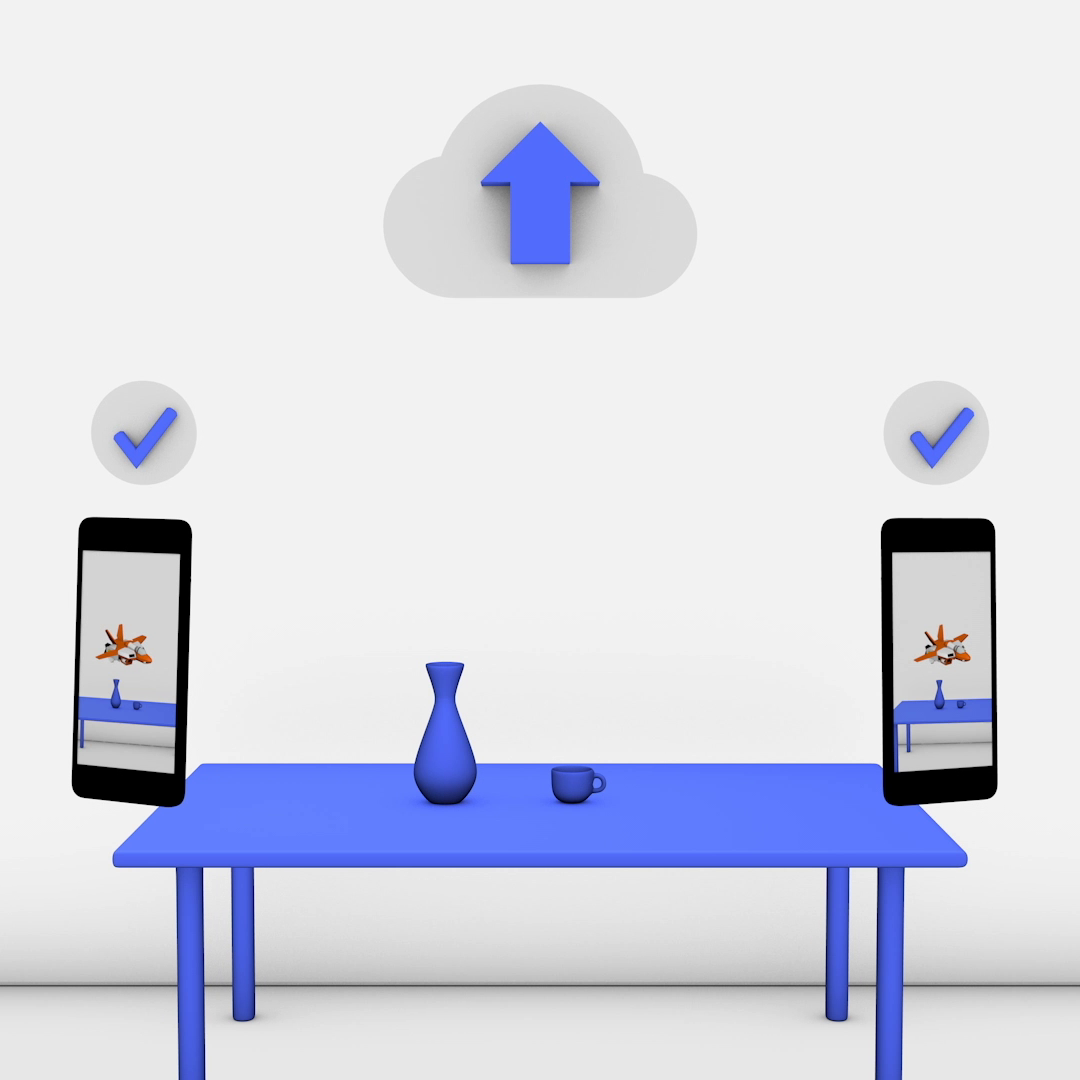
\includegraphics[width=0.45\textwidth]{./resources/images/cloud_anchors/resolving}}
		\caption{Funzionamento ad alto livello di Cloud Anchor API.}
		\label{fig:cloud}
	\end{figure}

	\section{Configurazione e utilizzo}
	Per implementare un'applicazione che utilizzi i Cloud Anchor è prima necessario creare un progetto in \textit{Google Cloud Platform} e abilitare il ARCore Cloud Anchor API per l'hosting, il salvataggio e il resolving degli anchor.
	\\
	\noindent
	La sessione ARCore deve essere impostata per poter utilizzare l'API Cloud Anchors, come descritto dal listing~\vref{lst:ca_session} tratto dalla documentazione ufficiale.
	\begin{center}
		\begin{minipage}{0.95\textwidth}
			\begin{lstlisting}[caption={Configurazione della modalità Cloud Anchor.}, label={lst:ca_session}, language=Kotlin]
			val config = Config(session)
			config.cloudAnchorMode = Config.CloudAnchorMode.ENABLED
			session.configure(config)
			\end{lstlisting}
		\end{minipage}
	\end{center}

	\subsection{Autenticazione}
	\label{subsec:auth}
	Se il cloud anchor deve poter avere processi host/resolve di durata massima 24 ore, come ad esempio per giochi virtuali multigiocatore, è necessaria un'autenticazione tramite chiave dell'app. Tale autenticazione si compie generando una \textit{API key} per il progetto cloud dal \textit{Google Cloud Console} e aggiungendola nel campo \verb|android:value| in un tag \verb|meta-data|, nel campo \verb|application| del file \verb|AndroidManifest.xml| dell'applicazione, come spiegato dal listing~\vref{lst:auth}.
	\begin{center}
		\begin{minipage}{0.95\textwidth}
			\begin{lstlisting}[caption={Autenticazione con API key.}, label={lst:auth}, language=xml, morekeywords={android:name, android:value}, keywordstyle={\color{NavyBlue}\bfseries}, alsodigit={-}, stringstyle={\color{ForestGreen}\ttfamily}, emph={meta-data},emphstyle={\color{OrangeRed}}]
			<meta-data
				android:name = "com.google.android.ar.API_KEY"
				android:value = "API_KEY"/>
			\end{lstlisting}
		\end{minipage}
	\end{center}

	\noindent
	Per cloud anchor che devono persistere per una durata compresa tra 1 e 365 giorni invece, è necessaria un'autenticazione tramite \textit{OAuth client}, che associa l'applicazione android al progetto di Google Cloud Platform. Tale autenticazione richiede una chiave \textit{SHA-1 fingerprint} che si può generare con il task \verb|signingReport| di Gradle.
	
	\subsection{Hosting}
	Il metodo \verb|hostCloudAnchorWithTtl(anchor:Anchor, ttlDays:Int)| della classe \verb|Session| permette di iniziare l'hosting di \verb|anchor| con una durata di \verb|ttlDays| giorni, un numero positivo compreso tra 1 e 365; per hosting con durata fino a 24 ore è invece necessaria l'invocazione del metodo \verb|hostCloudAnchor(anchor:Anchor)|. Entrambi i metodi restituiscono il nuovo anchor, con la stessa posizione di \verb|anchor| e con stato \verb|Anchor.CloudAnchorState.TASK_IN_PROGRESS|. Il listing~\vref{lst:hosting} tratto dal codelab \cite{codelab2021cloud} realizza l'hosting tramite un oggetto della classe wrapper \verb|CloudAnchorManager|.
	
	\begin{center}
		\begin{minipage}{0.95\textwidth}
			\begin{lstlisting}[caption={Hosting di un cloud anchor.}, label={lst:hosting}, language=Kotlin]
			val cloudAnchorManager : CloudAnchorManager = CloudAnchorManager();
				
			// Realizza l'hosting per l'anchor currentAnchor con durata 300 giorni
			cloudAnchorManager.hostCloudAnchor(session,currentAnchor,300,this::onHostedAnchorAvailable);
			\end{lstlisting}
		\end{minipage}
	\end{center}
	
	\subsection{Resolving}
	Il metodo \verb|resolveCloudAnchor(String cloudAnchorId)| della classe \verb|Session| compie il resolving, creando un anchor sulla base delle informazioni 3D inviate e comparate con la mappa 3D caricata durante l'hosting, per poter posizionare correttamente l'oggetto rispetto al dispositivo che sta compiendo il resolving.

	
\end{document}
	\documentclass[crop=false, class=book]{standalone}

%pacchetto per immagini
\usepackage{graphicx}
\usepackage{subfig}

\usepackage[italian]{varioref}
\usepackage{copyrightbox}
\usepackage{url}
\usepackage{siunitx}

\begin{document}
	\chapter{Geospatial API}
	
	L'API \textit{Geospatial} è una funzionalità aggiunta a maggio 2022 al framework ARCore, che utilizza i dati di \textit{Google Earth 3D} e \textit{Google Maps Street View} per creare contenuti AR basati sulla posizione geografica. L'API sfrutta il \textit{global localization}, il quale combina il \textit{VPS - Visual Positioning Service}, un servizio Google che analizza l'ambiente circostante attraverso la fotocamera per determinare la posizione, \textit{Street View}, che fornisce un database di immagini di luoghi, e il machine learning per migliorare la determinazione della posizione del dispositivo \cite{googleblog2019global}.
	\\
	\noindent
	Il Geospatial API compara le informazioni provenienti dalla fotocamera (figura~\vref{fig:geospatial_a}) e dai sensori del dispositivo, come il GPS, con miliardi di immagini 3D estratte tramite machine learning da Street View (figura~\vref{fig:geospatial_b}) per determinare la posizione e l'orientamento del dispositivo, per poi mostrare contenuti AR posizionati correttamente rispetto all'utente, come spiegato in \cite{googleblog2022geospatial}.
	
	\begin{figure}[tbph]
		\centering
		\subfloat[][\emph{Immagini della fotocamera del dispositivo} \label{fig:geospatial_a}]
		{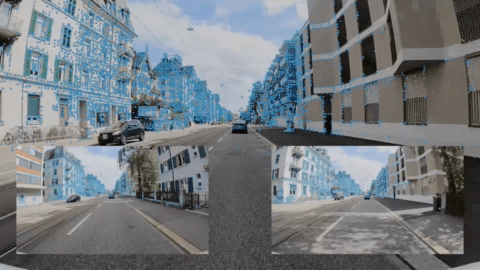
\includegraphics[width=0.47\textwidth]{./resources/images/geospatial/a.png}}  \quad
		\subfloat[][\emph{Confronto con immagini Street View} \label{fig:geospatial_b}]
		{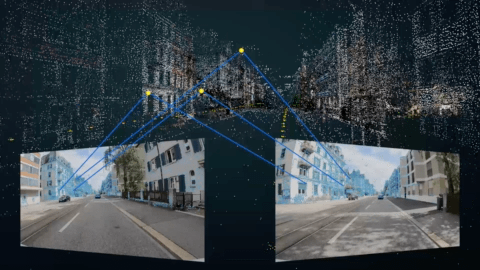
\includegraphics[width=0.47\textwidth]{./resources/images/geospatial/b.png}} \quad
		\caption{Ricostruzione delle funzionalità di Geospatial API.}
		\label{fig:geospatial}
	\end{figure}

	\section{Configurazione e utilizzo}
	La sessione ARCore deve abilitare l'utilizzo di Geospatial API, come descritto dal listing~\vref{lst:geo_session} tratto dalla documentazione ufficiale \cite{google2022geospatial}.
	
	\begin{center}
		\begin{minipage}{0.95\textwidth}
			\begin{lstlisting}[caption={Configurazione della modalità Geospatial API.}, label={lst:geo_session}, language=Kotlin]
			// Abilita il Geospatial API.
			session.configure(session.config.apply{ geospatialMode= Config.GeospatialMode.ENABLED})
			\end{lstlisting}
		\end{minipage}
	\end{center}
	
	\subsection{Configurazione di VPS}
	L'utilizzo di Visual Positioning System impone che l'app sia associata a un progetto Google Cloud Project con abilitato il ARCore API. \`E inoltre necessaria un'autenticazione tramite \textit{OAuth client}, oppure con \textit{API key}. Si veda il paragrafo~\vref{subsec:auth} del capitolo Cloud Anchor per specifiche su entrambi i tipi di autenticazione.
	\\
	Sono necessari inoltre i permessi per accedere alla posizione e ad internet per comunicare con il servizio online Geospatial API, da dichiarare nel campo \verb|manifest| del file \verb|AndroidManifest.xml|, come descritto dal listing~\vref{lst:geo_perm}.
	
	\begin{center}
		\begin{minipage}{0.95\textwidth}
			\begin{lstlisting}[caption={Richiesta di permessi per l'uso di Geospatial API.}, label={lst:geo_perm}, language=xml, morekeywords={android:name, android:value}, keywordstyle={\color{NavyBlue}\bfseries}, alsodigit={-}, stringstyle={\color{ForestGreen}\ttfamily}, emph={manifest, uses-permission},emphstyle={\color{OrangeRed}}]
			<manifest ...>
				<uses-permission android:name="android.permission.ACCESS_FINE_LOCATION"/>
				<uses-permission android:name="android.permission.ACCESS_COARSE_LOCATION"/>
				<uses-permission android:name="android.permission.INTERNET"/>
			</manifest>
			\end{lstlisting}
		\end{minipage}
	\end{center}

	\subsection{Calcolo della posizione}
	La posizione può essere presa da un oggetto della classe \verb|Earth|, ricevuto dalla sessione ARCore \verb|session|, come descritto dal listing~\vref{lst:geo_current}. Se l'oggetto di tipo \verb|Earth| ha stato \verb|TrackingState.TRACKING|, la posizione può essere ottenuta tramite un oggetto di tipo \verb|GeospatialPose|, che contiene la latitudine e la longitudine, l'altitudine e un'approssimazione della direzione verso cui il dispositivo è rivolto.
	\begin{center}
		\begin{minipage}{0.95\textwidth}
			\begin{lstlisting}[caption={Calcolo della posizione corrente.}, label={lst:geo_current}, language=Kotlin]
			val earth = session.earth
			// Verifico che sia in stato TRACKING
			if (earth?.trackingState == TrackingState.TRACKING) {
				val cameraGeospatialPose : GeospatialPose = earth.cameraGeospatialPose
				
				// Salvataggio della latitudine in gradi
				val latitude : Double = cameraGeospatialPose.latitude
				// Salvataggio della longitudine in gradi
				val longitude : Double = cameraGeospatialPose.longitude
				// Salvataggio dell'altitudine in metri
				val elevation : Double = cameraGeospatialPose.altitude
				// Salvataggio dell'orientamento in gradi
				val heading : Double = cameraGeospatialPose.heading
			}
			\end{lstlisting}
		\end{minipage}
	\end{center}
	\noindent
	L'oggetto \verb|GeospatialPose| specifica anche l'accuratezza $A$ dei dati ricevuti, tramite i metodi \verb|getHeadingAccuracy()|, \verb|getHorizontalAccuracy()| e \verb|getVerticalAccuracy()|. I valori restituiti dai metodi hanno stessa unità di misura dei valori stimati $E$ di cui specificano la precisione, cioè gradi per la latitudine, la longitudine e l'orientamento e metri per l'altitudine, e specificano che la posizione reale $R$ è compresa con una probabilità del $68\%$ nell'intervallo:
	\[
		R \in [E-A, E+A].
	\] 
	Ad esempio, se il metodo \verb|GeospatialPose.getHeading()| restituisce il valore $E = \SI{60}{\degree}$ e il metodo \verb|GeospatialPose.getHeadingAccuracy()| ritorna una precisione di $A = \SI{10}{\degree}$, il valore reale sarà con probabilità del $68\%$ nell'intervallo $R \in [\SI{50}{\degree}, \SI{70}{\degree}]$. Un valore alto di accuratezza quindi garantisce una precisione minore.

	\subsection{Posizionamento di un anchor Geospatial}
	Per il posizionamento di un anchor, i valori di latitudine e longitudine devono essere dati rispettando le specifiche WGS84, mentre l'altitudine è definita come la distanza in metri dall'elissoide definito dallo stesso standard. 
	L'orientamento dell'anchor invece viene fatto con l'utilizzo di un quaternione \verb|(qx,qy,qz,qw)|. Si veda il listing~\vref{lst:geo_pos} per un esempio di creazione dell'anchor.
	\begin{center}
		\begin{minipage}{0.95\textwidth}
			\begin{lstlisting}[caption={Posizionamento di anchor Geospatial.}, label={lst:geo_pos}, language=Kotlin]
			if (earth.trackingState == TrackingState.TRACKING) {
				val anchor = earth.createAnchor (
				/* Valori della posizione */
				latitude,longitude,altitude,
				/* Valori della rotazione */
				qx,qy,qz,qw)
				// ...
			}
			\end{lstlisting}
		\end{minipage}
	\end{center}
	\noindent
	L'altitudine dell'anchor, se esso viene posizionato vicino all'utente, può avere lo stesso valore dell'altitudine restituita dal metodo \verb|GeospatialPose.getAltitude()|. Se invece l'anchor deve avere un'altitudine diversa da quella dell'utente, essa può essere ricavata dall'API Google Maps, forzando la prospettiva 2D e convertendo il valore restituito, basato sullo standard EGM96, nella codifica WGS84.
	
	
	
	
	
	
	
	
	
	
\end{document}
	
	\backmatter
	\documentclass[crop=false]{standalone}


\usepackage[autostyle,italian=guillemets]{csquotes}
\usepackage[style=numeric,citestyle=numeric-comp,backend=biber]{biblatex}

\addbibresource{bibliografia.bib}

\begin{document}
	\printbibliography[heading=bibintoc]
\end{document}
	
	
\end{document}
